\documentclass{beamer}
\usetheme{Madrid}
\usepackage{thesis-style}

\begin{document}

% Título de la tesis
\title[Tesis de grado]{Modelo elástico de replicación de operadores para un sistema de procesamiento de \textit{stream} en tiempo real}

% Grado
\subtitle{Tesis de grado}

% Autores
\author[Daniel Wladdimiro C.]{Daniel Wladdimiro Cottet\\\scriptsize{Profesor guía: Dr. Nicol\'as Hidalgo C.}\\\scriptsize{Profesora co-guía: Dra. Erika Rosas O.}}

% Institución
\institute[UdeSantiago]
{
  Departamento de Ingenier\'ia Inform\'atica\\
  Universidad de Santiago de Chile
 }

% Logo
\addtobeamertemplate{frametitle}{}{
    \begin{textblock*}{100mm}(0.93\textwidth,-1.2cm)
   
\includegraphics[scale=0.022]{images/LogoUsach.png}
    \end{textblock*}
}

% Fecha
\date[Santiago, 2015]{\scriptsize{Santiago - Chile\\2015}}

% Portada
\begin{frame}
  \titlepage
\end{frame}

\begin{frame}[t]{Contenidos}{\textcolor{UniBlue}{.}}
	\tableofcontents
\end{frame}

\section{Introducción}
\subsection*{Antecedentes y motivación}

\begin{frame}{Introducción}{Antecedentes y motivación}
La interacción entre los distintos usuarios gener\'o una gran cantidad de datos, la cual se puede procesar y obtener información relevante
\begin{figure}
  \center
    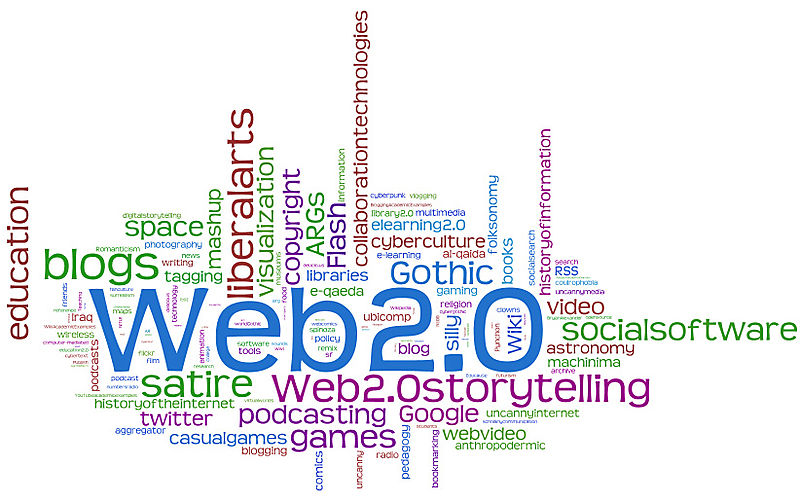
\includegraphics[scale=0.35]{images/Web.jpg}
\end{figure}
\end{frame}

\begin{frame}{Introducción}{Antecedentes y motivación}
\begin{itemize}
\item Sistemas de procesamiento capaces de lidiar con restricciones de temporalidad
\item Manejo de grandes flujos de datos en tiempo real
\item Debido a la necesidad de respuestas rápidas y actualizadas
\item Apoyo en la toma de decisiones
\item Por ejemplo:
	\begin{itemize}
	%\item Análisis de sentimientos de los mensajes de usuarios 
	\item Predicciones del comportamiento en la bolsa de valores
	\item Recopilación de información en caso de emergencia
	\item Seguridad en redes 
	\end{itemize}
\end{itemize}
\end{frame}

\begin{frame}{Introducción}{Antecedentes y motivación}
\begin{itemize}
\item Tipos de sistemas de procesamiento de \textsl{stream}
	\begin{itemize}
	\item S4
	\item Storm
	\item Samza
	\end{itemize}
\item \textsl{Problemas}
	\begin{itemize}
	\item Poca adaptaci\'on del sistema en tiempo de ejecución
	\item Posibles problemas de distribución de carga
	\item Baja en el rendimiento
	\item Pérdida de recursos e información
	\end{itemize}
\end{itemize}
\end{frame}

\subsection*{Descripción del problema}

\begin{frame}{Introducción}{Descripción del problema}
\begin{block}{}
	Dado el carácter estático del grafo de procesamiento en tiempo de ejecución y el carácter altamente dinámico del tráfico, pueden surgir problemas de balance de carga entre los operadores de la topología, sobrecargando alguno de estos y comprometiendo el rendimiento del sistema.
\end{block}
\end{frame}
\section{Balance de carga}
\subsection*{Perspectivas de balance de carga}

\addtocounter{framenumber}{-1}
\begin{frame}[t]{Contenidos}{\textcolor{UniBlue}{.}}
	\tableofcontents[currentsection]
\end{frame}

\begin{frame}{Balance de carga}{Perspectivas de balance de carga}
\begin{itemize}
\item Perspectivas al problema de balance de carga en procesamiento de \textsl{stream}
\begin{itemize}
	\item Recursos físicos
	\item Grafo de operadores
\end{itemize}
\item Para la optimización del sistema, se presentan dos enfoques \cite{Dong06schedulingalgorithms}
\begin{itemize}
	\item Estático
	\item Dinámico
\end{itemize}
\end{itemize}
\end{frame}

\begin{frame}{Balance de carga}{Enfoque dinámico}
\begin{itemize}
\item En el estado del sistema
\item Las variables y estados de cada uno de sus atributos
\item Cambios en el sistema ante una anomalía
\item Tipos de modelo para las soluciones:
\begin{itemize}
	\item Reactivo \cite{GulisanoJPSV12}
	\item Predictivo \cite{NguyenSGSW13}
\end{itemize}
\end{itemize}
\end{frame}

\subsection*{Técnicas de balance de carga}
\begin{frame}{Balance de carga}{Técnicas de balance de carga}
\begin{itemize}
\item Existes diversas técnicas que permiten balancear la carga, como:
\begin{itemize}
	\item Planificación determinista \cite{XuCTS14, DongTS07}
	\item Descarte de eventos \cite{SheuC09}
	\item Migración \cite{XingZH05}
	\item Fisión \cite{GulisanoJPSV12, IshiiS11, GedikSHW14, FernandezMKP13}
\end{itemize}
\end{itemize}
\end{frame}
\section{Solución propuesta}
\subsection*{Objetivos y alcance del proyecto}

\addtocounter{framenumber}{-1}
\begin{frame}[t]{Contenidos}{\textcolor{UniBlue}{.}}
	\tableofcontents[currentsection]
\end{frame}

\begin{frame}{Solución propuesta}{Objetivos y alcance del proyecto}

\begin{alertblock}{Objetivo general}
Dise\~no, construcción y evaluaci\'on de un modelo elástico de replicación de operadores para un sistema de procesamiento de \textit{stream} en tiempo real
\end{alertblock}

\pause
\begin{enumerate}
	\item Dise\~nar e implementar un algoritmo reactivo que permita analizar en el momento la carga de los operadores
	\pause
	\item Dise\~nar e implementar un algoritmo de predicci\'on que permita estimar la carga de los operadores
	\pause
	\item Dise\~nar e implementar un algoritmo que permita la administraci\'on del número de operadores del grafo de procesamiento de forma el\'astica
	\pause
	\item Dise\~nar y construir experimentos que permitan validar la hip\'otesis formulada
	\pause
	\item Evaluar y analizar el rendimiento del modelo a trav\'es de aplicaciones generadas sobre un sistema de procesamiento de \textit{stream}
\end{enumerate}
\end{frame}

\begin{frame}{Solución propuesta}{Objetivos y alcance del proyecto}
Los alcances del proyecto se encuentran:
\begin{itemize}
	\item Evaluación sobre un sólo sistema de procesamiento de \textsl{stream}
	\item Datos emitidos de la fuente de datos son homogéneos
	\item Distribución de carga a nivel de operadores y no de máquinas
	\item No garantiza completo procesamiento de los datos
	\item Costo de comunicación de manera igualitaria para todos los operadores
\end{itemize}
\end{frame}
\section{Diseño del modelo elástico}
\subsection*{Análisis del modelo elástico}

\addtocounter{framenumber}{-1}
\begin{frame}[t]{Contenidos}{\textcolor{UniBlue}{.}}
	\tableofcontents[currentsection]
\end{frame}

\begin{frame}[t]{Diseño del modelo elástico}{Análisis del modelo elástico}
\begin{itemize}
\item Recursos lógicos del sistema según el enfoque dinámico
\item Bajo overhead $\rightarrow$ Escalable
\item Técnica de fisión
\end{itemize}

\begin{picture}(0,80)
	\put(60,0){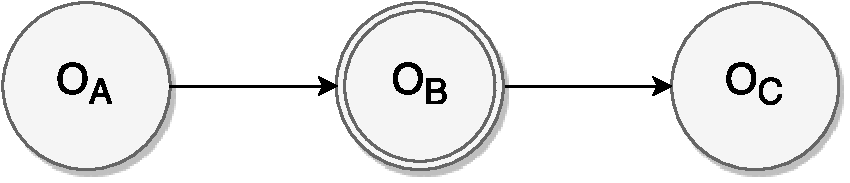
\includegraphics[scale=.5]{images/EjReplicacion-I.pdf}}
\end{picture}

\end{frame}

\addtocounter{framenumber}{-1}
\begin{frame}[t]{Diseño del modelo elástico}{Análisis del modelo elástico}
\begin{itemize}
\item Recursos lógicos del sistema según el enfoque dinámico
\item Bajo overhead $\rightarrow$ Escalable
\item Técnica de fisión
\end{itemize}

\begin{picture}(0,120)
	\put(60,0){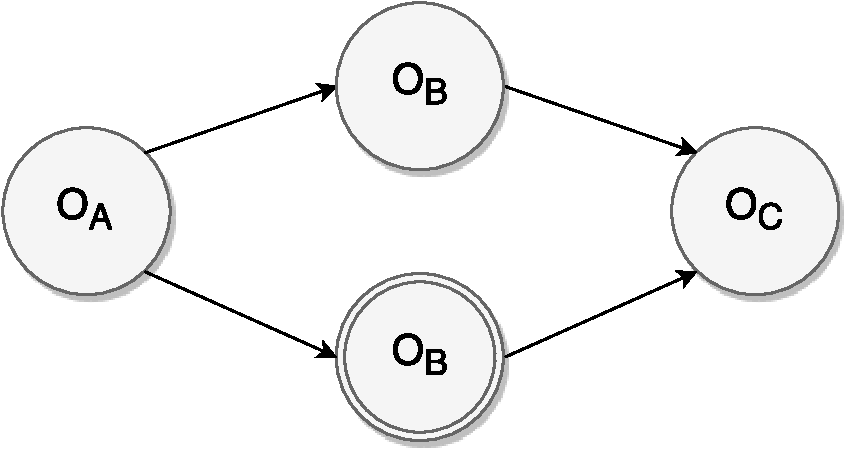
\includegraphics[scale=.5]{images/EjReplicacion-II.pdf}}
\end{picture}

\end{frame}

\addtocounter{framenumber}{-1}
\begin{frame}[t]{Diseño del modelo elástico}{Análisis del modelo elástico}
\begin{itemize}
\item Recursos lógicos del sistema según el enfoque dinámico
\item Bajo overhead $\rightarrow$ Escalable
\item Técnica de fisión
\end{itemize}

\begin{picture}(0,150)
	\put(60,0){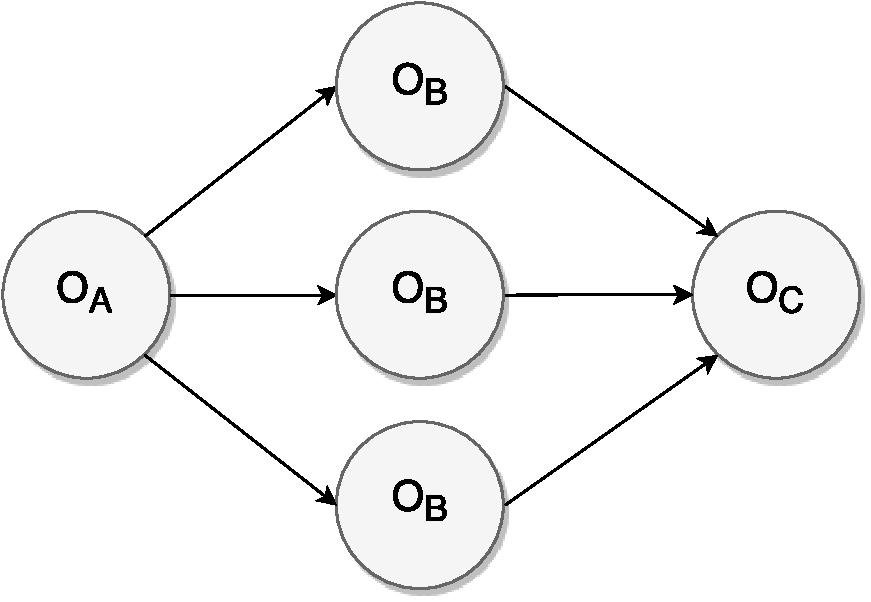
\includegraphics[scale=.5]{images/EjReplicacion-III.pdf}}
\end{picture}

\end{frame}

\begin{frame}{Diseño del modelo elástico}{Análisis del modelo elástico}
\begin{itemize}
\item Umbrales $\rightarrow$ Tasa de rendimiento $\rho$
	\begin{itemize}
		\item $\rho = \frac{\lambda}{s \mu}$
	\end{itemize}
\end{itemize}

\begin{figure}[!hb]
	\centering
	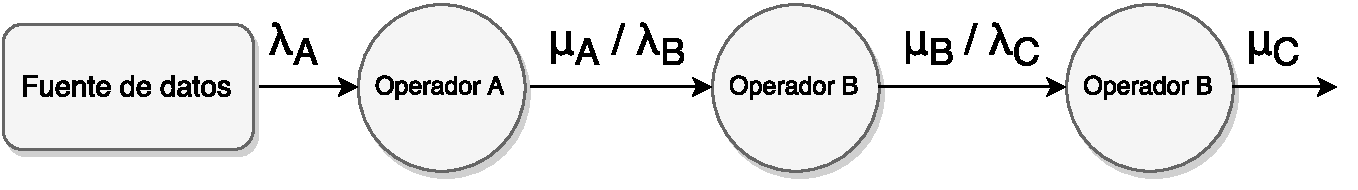
\includegraphics[scale=0.35]{images/AnalisisTeoriaColas.pdf}
\end{figure}

\begin{itemize}
\item Enfoque dinámico y elasticidad
\begin{itemize}
	\item Estados: ocioso, estable e inestable
\end{itemize}
\item Dos tipos de algoritmos: reactivo y predictivo
\item Recolector de datos y administrador de réplicas
\end{itemize}
\end{frame}

\begin{frame}{Diseño del modelo elástico}{Análisis del modelo elástico}
\begin{figure}[ht!]
  \centering
    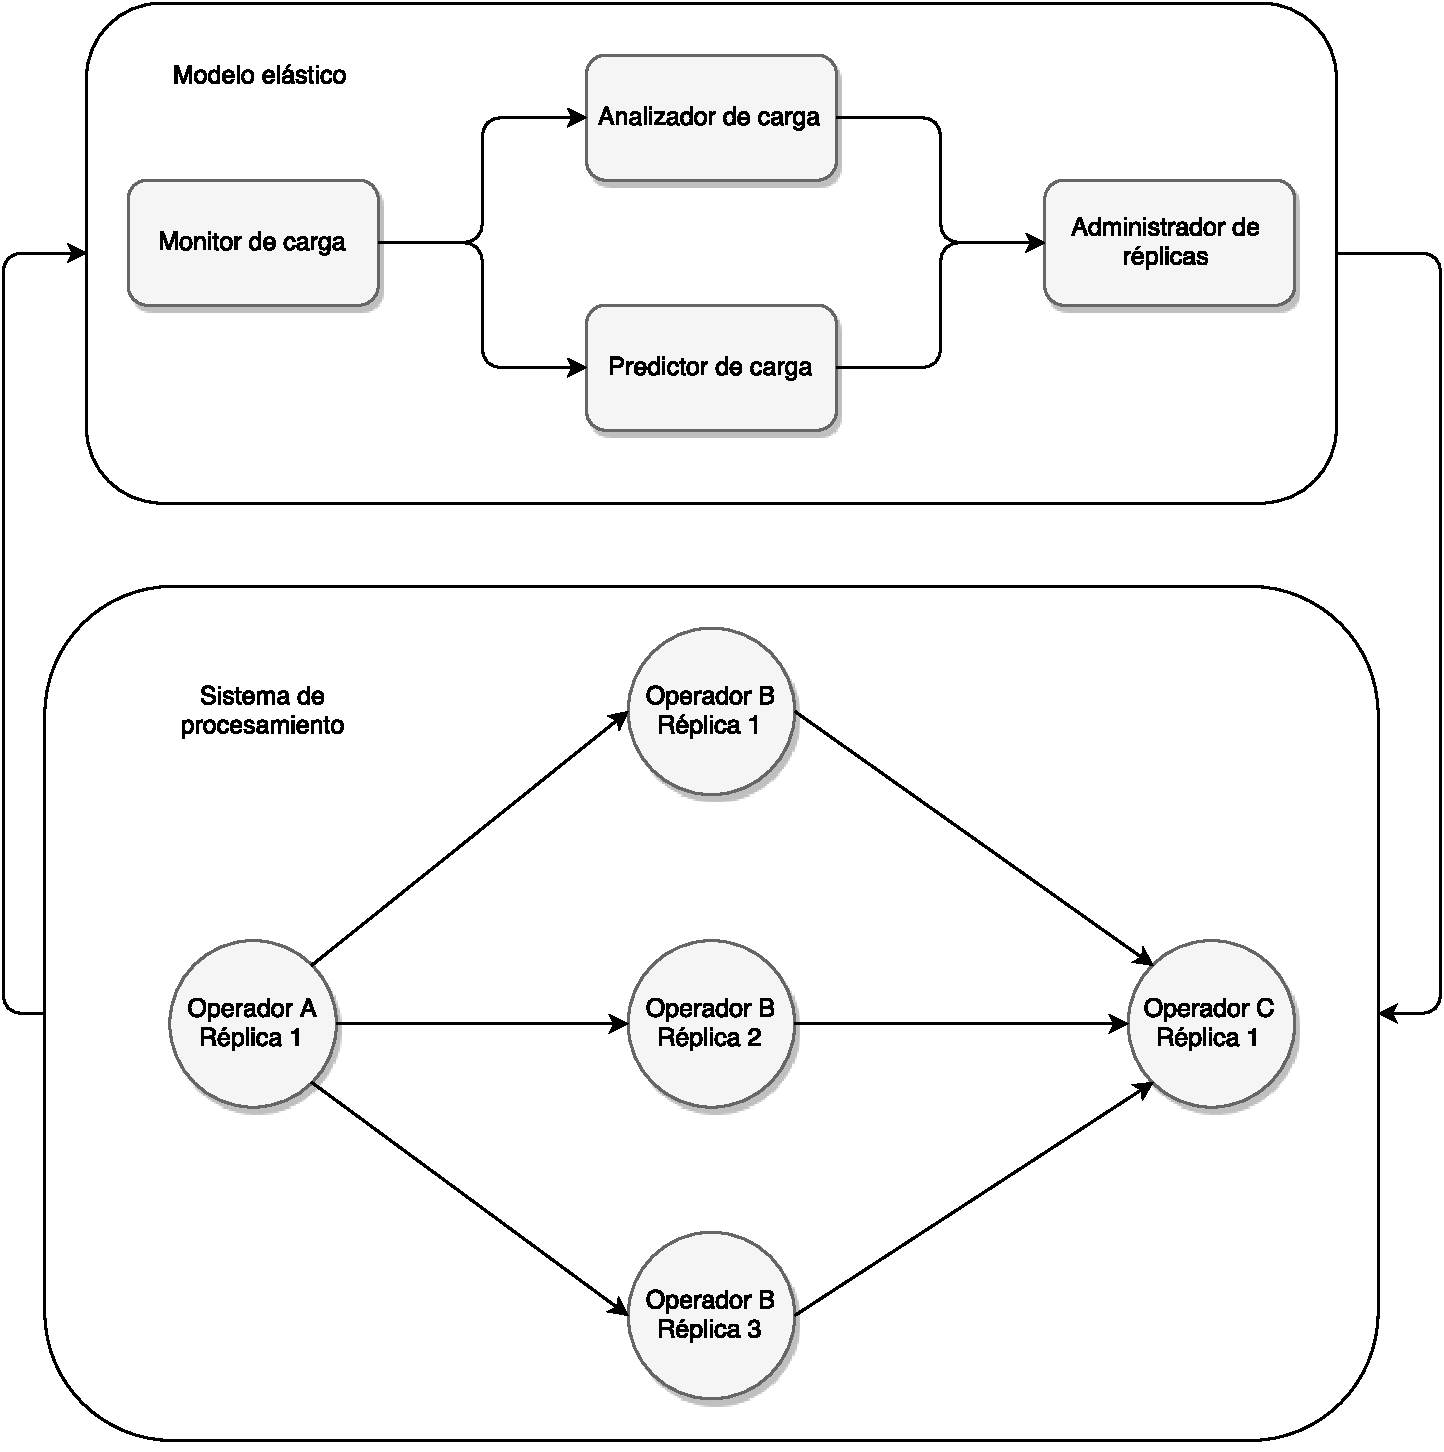
\includegraphics[scale=0.3]{images/Diagrama.pdf}
\end{figure}
\end{frame}

\subsection*{Recolección de los datos}
\begin{frame}{Diseño del modelo elástico}{Recolección de los datos}
El monitor de carga es el encargado de recolectar los datos
\begin{itemize}
	\item Algoritmo reactivo $\rightarrow$ Tasa de procesamiento $\rho$
	\begin{itemize}
		\item Tasa de rendimiento $\mu$ es homogénea
		\item Ventana de tiempo $T_r$
	\end{itemize}
	\item Algoritmo predictivo $\rightarrow$ Historial
	\begin{itemize}
		\item Ventanas de tiempo de $T$
		\item $n$ muestras
		\item Ventana de tiempo $T_p$
	\end{itemize}
\end{itemize}

\end{frame}

\subsection*{Algoritmo reactivo}
\begin{frame}{Diseño del modelo elástico}{Algoritmo reactivo}
\begin{itemize}
\item Análisis del estado del operador $\rightarrow$ Período de tiempo
\item Tasa de rendimiento $\rho$
\end{itemize}
\hspace{1cm}
\begin{tabular}{c c}
	$\rho > 1$ & Inestable \\
	$1 \geqslant \rho \geqslant 0.5$ & Estable \\
	$\rho < 0.5$ & Ocioso
\end{tabular}
\end{frame}

\begin{frame}{Diseño del modelo elástico}{Algoritmo reactivo}
\begin{itemize}
\item Comportamiento de la tasa de rendimiento
\end{itemize}
\begin{figure}[ht!]
  \centering
    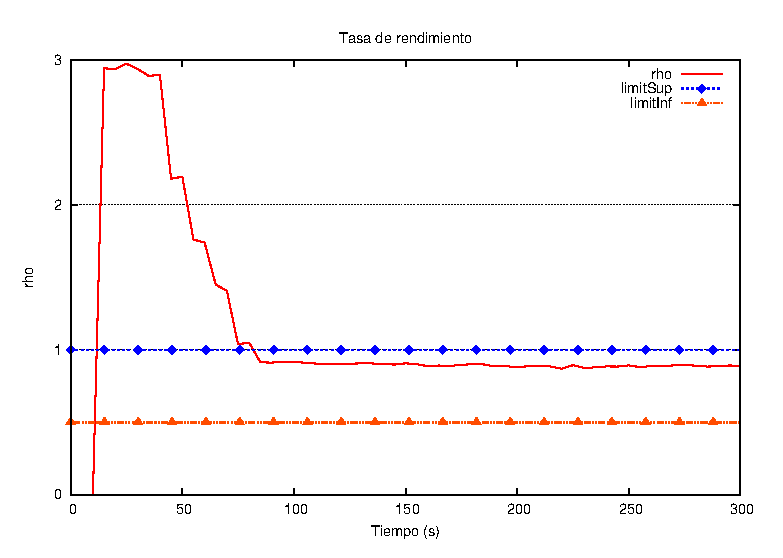
\includegraphics[scale=0.6]{images/Umbrales.eps}
\end{figure}
\end{frame}

\subsection*{Algoritmo predictivo}
\begin{frame}{Diseño del modelo elástico}{Algoritmo predictivo}
\begin{itemize}
	\item Definir muestras en tiempos discretos, las cuales cambian con el tiempo según un proceso estocástico
	\item Determinar los estados finitos que se utilizan para la conformación de la cadena
	\item Obtener una cantidad representativa de muestras para la construcción de la cadena de Markov en el período analizado
\end{itemize}

\begin{figure}[ht!]
  \centering
    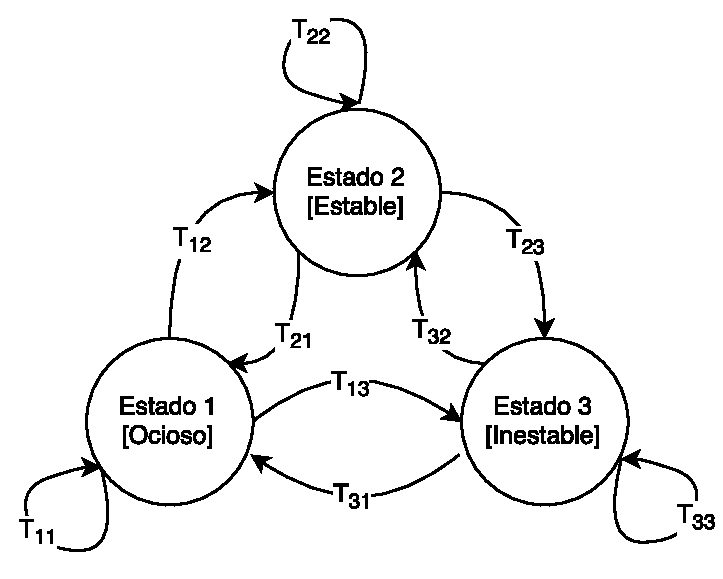
\includegraphics[scale=0.35]{images/CadenaMarkovPredictiva.pdf}
\end{figure}

\end{frame}


\begin{frame}{Diseño del modelo elástico}{Algoritmo predictivo}
\begin{itemize}
	\item Construcción de la matriz de transición
		\begin{itemize}
			\item La transición de estados de un período a otro
		\end{itemize}
\end{itemize}
\vspace{-1cm}
\begin{center}
\begin{align*}
	P =
	\begin{bmatrix}
		T_{1,1} & T_{1,2} & T_{1,3} \\
		T_{2,1} & T_{2,2} & T_{2,3} \\
		T_{3,1} & T_{3,2} & T_{3,3}
	\end{bmatrix}	
\end{align*}
\end{center}

\begin{itemize}		
	\item Ecuación de Chapman-Kolmogórov $\rightarrow$ Distribución Estacionaria
	\begin{itemize}
		\item Comportamiento a futuro de la Cadena de Markov
	\end{itemize}
\end{itemize}
\vspace{-1cm}
\begin{center}
\begin{align*}
\begin{bmatrix}
	\Pi_1 & \Pi_2 & \Pi_3
\end{bmatrix} _{(t+1)}
\end{align*}
\end{center}
\vspace{-0.5cm}
\begin{itemize}		
	\item $\sigma(\Pi_1, \Pi_2, \Pi_3) > 0.25$
	\begin{itemize}
		\item No posee incertidumbre
		\item En caso contrario, no es un comportamiento determinante
	\end{itemize}
\end{itemize}
\end{frame}

\subsection*{Administración del sistema}
\begin{frame}{Diseño del modelo elástico}{Administración del sistema}
\begin{itemize}
\item Administración de réplicas de un operador
\item Recursos disponibles de la máquina
\item Según el período se ejecuta
\begin{itemize}
	\item $T_p \rightarrow $ Algoritmo predictivo
	\begin{itemize}
		\item Menor frecuencia
		\item Mayor cómputo
		\item Modifica mayor cantidad de réplicas
	\end{itemize}
	\item $T_r \rightarrow $ Algoritmo reactivo
	\begin{itemize}
		\item Dos alertas $\rightarrow$ Modifica
	\end{itemize}
\end{itemize}
\end{itemize}
\end{frame}
\section{Experimentos y evaluación}
\subsection*{Implementación del sistema}

\addtocounter{framenumber}{-1}
\begin{frame}[t]{Contenidos}{\textcolor{UniBlue}{.}}
	\tableofcontents[currentsection]
\end{frame}

\begin{frame}{Experimentos y evaluación}{Implementación del sistema}
\begin{itemize}
\item SPS S4 $\rightarrow$ Modifica el código fuente
	\begin{itemize}
		\item Cantidad de eventos entrantes y salientes de cada PE
	\end{itemize}
\item Distribución de la carga según la cola
	\begin{itemize}
		\item Política según el largo de la cola
	\end{itemize}
\end{itemize}

\begin{figure}
  \center
    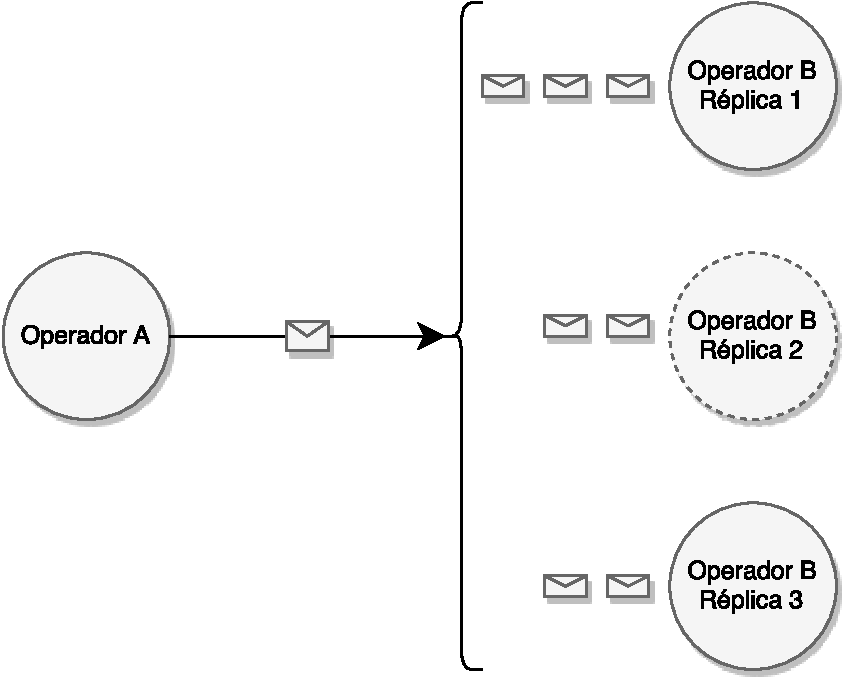
\includegraphics[scale=0.35]{images/DistribucionCarga-I.pdf}
\end{figure}
\end{frame}

\addtocounter{framenumber}{-1}
\begin{frame}{Experimentos y evaluación}{Implementación del sistema}
\begin{itemize}
\item SPS S4 $\rightarrow$ Modifica el código fuente
	\begin{itemize}
		\item Cantidad de eventos entrantes y salientes en cada PE
	\end{itemize}
\item Distribución de la carga según la cola
	\begin{itemize}
		\item Política según el largo de la cola
	\end{itemize}
\end{itemize}

\begin{figure}
  \center
    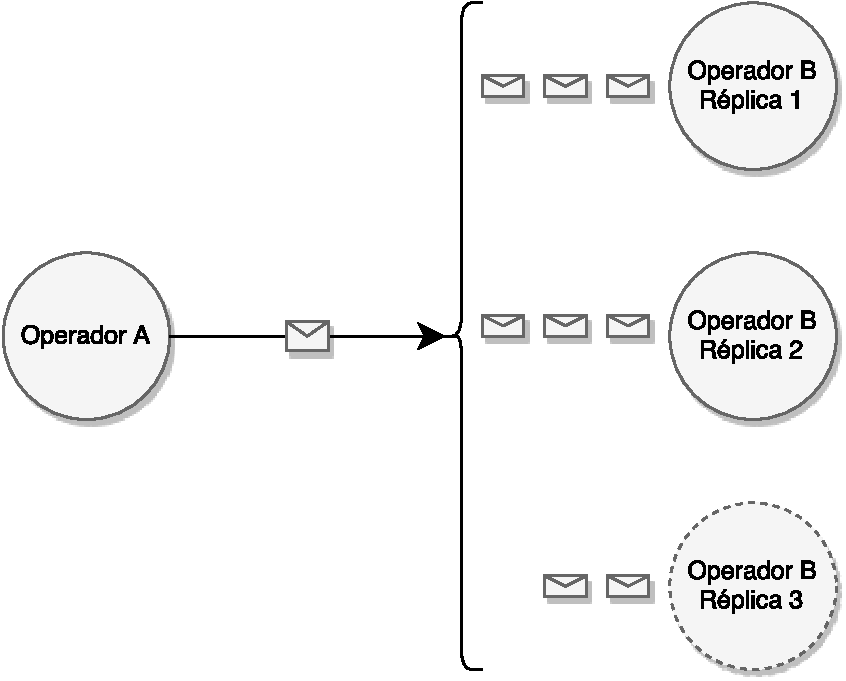
\includegraphics[scale=0.35]{images/DistribucionCarga-II.pdf}
\end{figure}
\end{frame}

\addtocounter{framenumber}{-1}
\begin{frame}{Experimentos y evaluación}{Implementación del sistema}
\begin{itemize}
\item SPS S4 $\rightarrow$ Modifica el código fuente
	\begin{itemize}
		\item Cantidad de eventos entrantes y salientes en cada PE
	\end{itemize}
\item Distribución de la carga según la cola
	\begin{itemize}
		\item Política según el largo de la cola
	\end{itemize}
\end{itemize}

\begin{figure}
  \center
    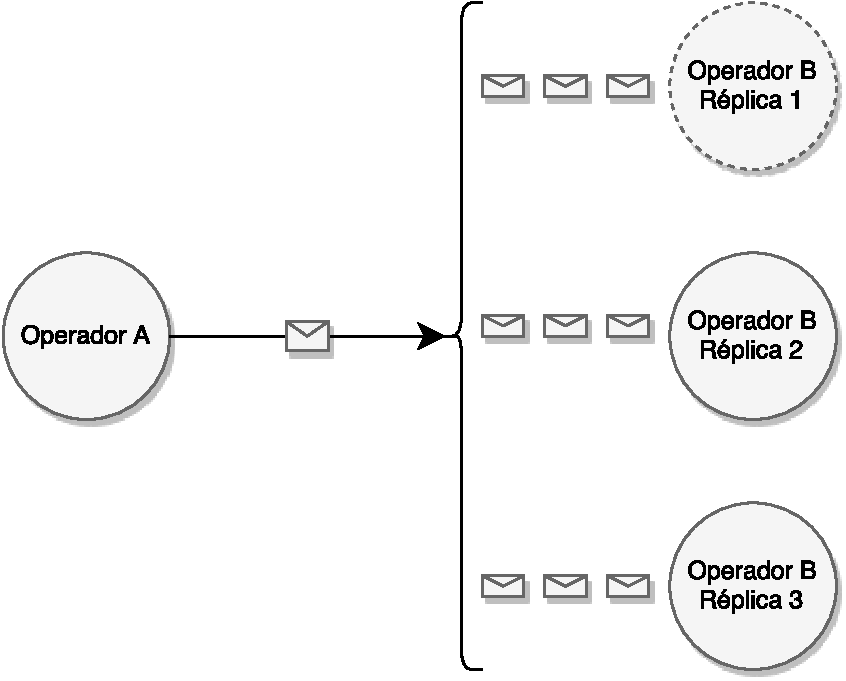
\includegraphics[scale=0.35]{images/DistribucionCarga-III.pdf}
\end{figure}
\end{frame}

\subsection*{Diseño de los experimentos}
\begin{frame}{Experimentos y evaluación}{Diseño de los experimentos}
\begin{itemize}
\item Dos tipo de aplicaciones
	\begin{itemize}
		\item Aplicación funcional
		\item Aplicación sintética
	\end{itemize}
\item Generación de stream
\begin{itemize}
	\item 4.5 millones de tweets
	\item 27-28 de Febrero y 1-2 de Marzo de 2010
	\item Inglés, español y portugués
	\item Interacción entre usuarios durante el terremoto del 27 de Febrero en Chile
\end{itemize}
\end{itemize}
\end{frame}

\begin{frame}{Experimentos y evaluación}{Diseño de los experimentos}
\begin{itemize}
	\item Aplicación funcional: Análisis de \textit{tweets} en escenarios de desastres naturales
	\begin{itemize}
		\item Validación del modelo dado un escenario aplicado
	\end{itemize}
\end{itemize}
\begin{figure}[!hb]
	\centering
		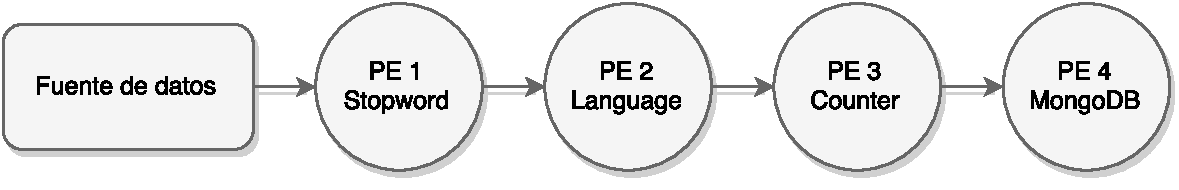
\includegraphics[scale=0.55]{images/App1.pdf}
\end{figure}
\end{frame}

\begin{frame}{Experimentos y evaluación}{Diseño de los experimentos}
\begin{itemize}
	\item Aplicación sintética
	\begin{itemize}
		\item Costos del uso del monitor
	\end{itemize}
\end{itemize}
\begin{figure}[!ht]
	\centering
		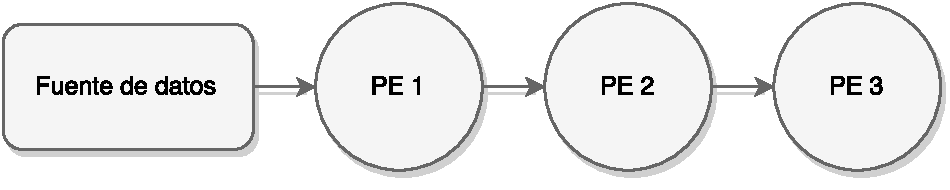
\includegraphics[scale=0.65]{images/App3.pdf}
\end{figure}
\begin{itemize}
	\item Período de tiempo que duerme la hebra asignada al PE
	\begin{itemize}
		\item Basadas del promedio de ejecución de operadores
	\end{itemize}
\end{itemize}
\begin{table}[!ht]
\footnotesize
\centering
\begin{tabular}{| c | c |}
\hline
PE & Tiempo (ms) \\ \hline
1 & 20 \\
2 & 30 \\
3 & 15 \\\hline
\end{tabular}
\end{table}
\end{frame}

\subsection*{Evaluación}
\begin{frame}{Experimentos y evaluación}{Evaluación}
\begin{itemize}
\item Para la ejecución de todos los experimentos se ha utilizado una máquina con un Intel Xeon CPU E5-2650 v2 de 2.60 GHz, 32 GB de RAM y SO Ubuntu 14.04.2 LTS

\item Para la evaluación de la primera aplicación se han realizado dos experimentos con distintos tiempos de ejecución:
\begin{itemize}
\item En el primer experimento es 60 minutos
\item Y en el segundo experimento es 10 minutos
\end{itemize}

\item Para la evaluación de la segunda aplicación se ha realizado un experimento
\begin{itemize}
	\item Envío constante de 100 eventos/s
	\item Tiempo de ejecución de 15 minutos
\end{itemize}

\item Cada uno de los experimentos se prueba con y sin modelo elástico

\end{itemize}
\end{frame}

%%% App 1 - Dynamic %%%

\begin{frame}{Experimentos y evaluación}{Aplicación funcional - Experimento 1 - Rendimiento y cantidad de réplicas}

\begin{itemize}
\item 96 eventos/segundo con uso del modelo \textit{vs} 16 eventos/segundo sin uso del modelo
\item Incremento de 5 veces más eventos/segundo
\end{itemize}

\begin{multicols}{2}
\begin{figure}[p]
	\centering
	{\scriptsize Con uso del modelo elástico\\}
	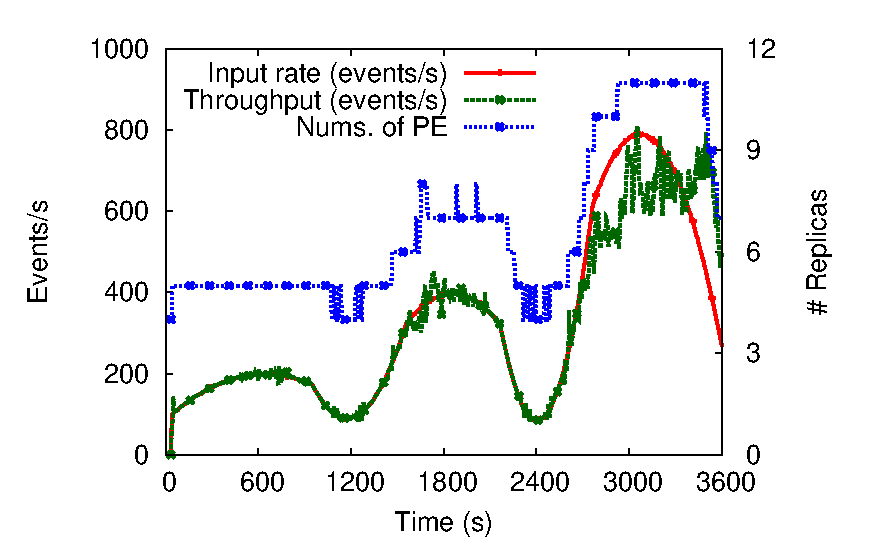
\includegraphics[scale=0.4]{images/exp/app1/dynamic/adaptative/exp1-processSystem.eps}
\end{figure}

\begin{figure}[p]
	\centering
	{\scriptsize Sin uso del modelo elástico\\}
	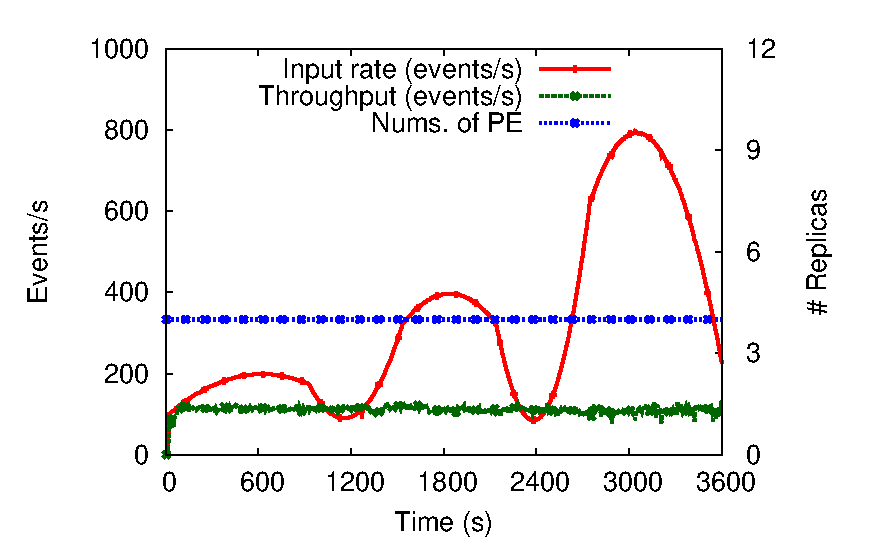
\includegraphics[scale=0.4]{images/exp/app1/dynamic/baseline/exp1-processSystem.eps}
\end{figure}
\end{multicols}
\end{frame}

\begin{frame}{Experimentos y evaluación}{Aplicación funcional - Experimento 1 - Cantidad total de eventos procesados}

\begin{itemize}
\item 1.139.537 eventos procesados con uso del modelo \textit{vs} 467.466 eventos procesados sin uso del modelo
\item Incremento de 2 veces la cantidad de eventos procesados
\end{itemize}

\begin{multicols}{2}
\begin{figure}[p]
	\centering
	{\scriptsize Con uso del modelo elástico\\}
	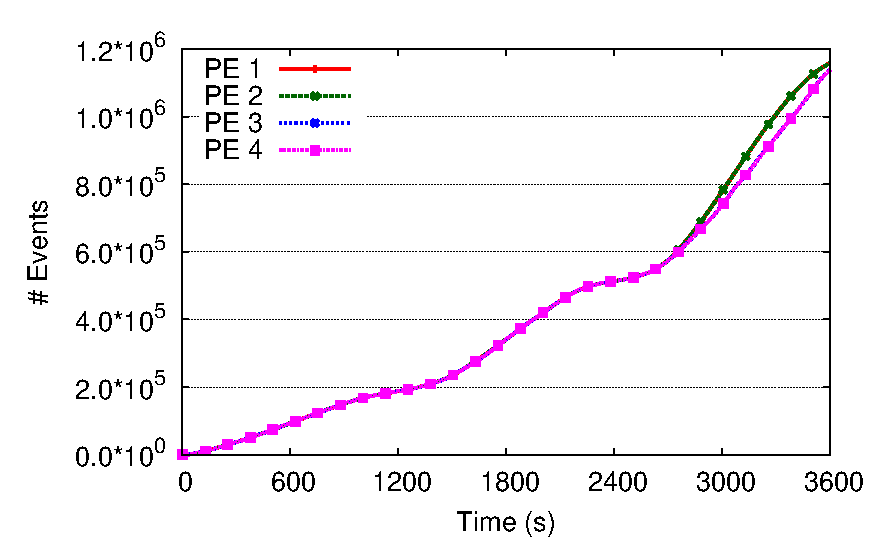
\includegraphics[scale=0.4]{images/exp/app1/dynamic/adaptative/exp1-eventCount.eps}
\end{figure}

\begin{figure}[p]
	\centering
	{\scriptsize Sin uso del modelo elástico\\}
	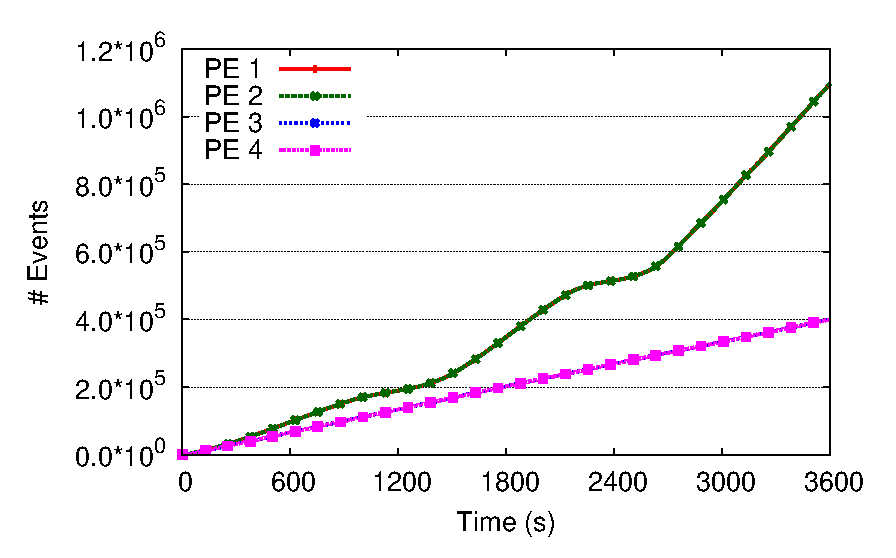
\includegraphics[scale=0.4]{images/exp/app1/dynamic/baseline/exp1-eventCount.eps}
\end{figure}
\end{multicols}
\end{frame}

%%% App 1 - Dynamic %%%
\begin{frame}{Experimentos y evaluación}{Aplicación funcional - Experimento 2 - Rendimiento y cantidad de réplicas}

\begin{itemize}
\item 72 eventos/segundo con uso del modelo \textit{vs} 19 eventos/segundo sin uso del modelo
\item Incremento de 3 veces más eventos/segundo
\end{itemize}

\begin{multicols}{2}
\begin{figure}[p]
	\centering
	{\scriptsize Con uso del modelo elástico\\}
	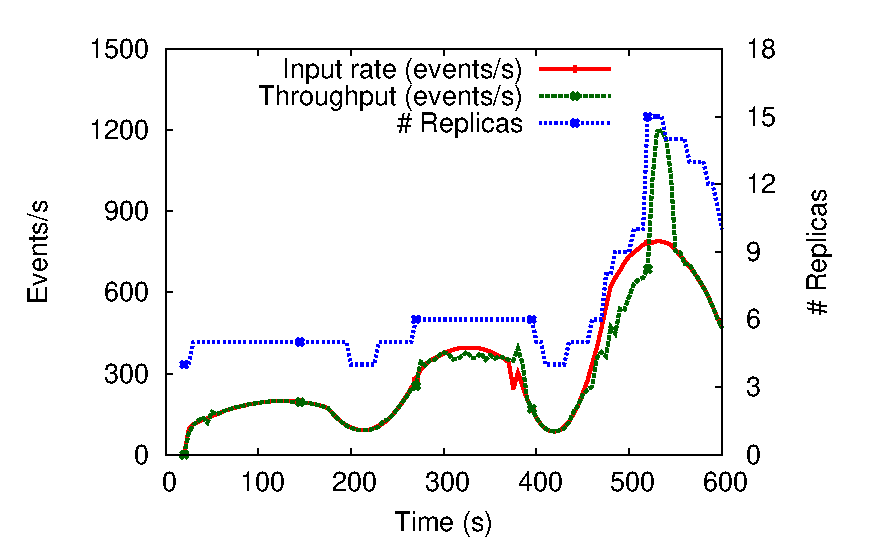
\includegraphics[scale=0.4]{images/exp/app1/dynamic/adaptative/exp2-processSystem.eps}
\end{figure}

\begin{figure}[p]
	\centering
	{\scriptsize Sin uso del modelo elástico\\}
	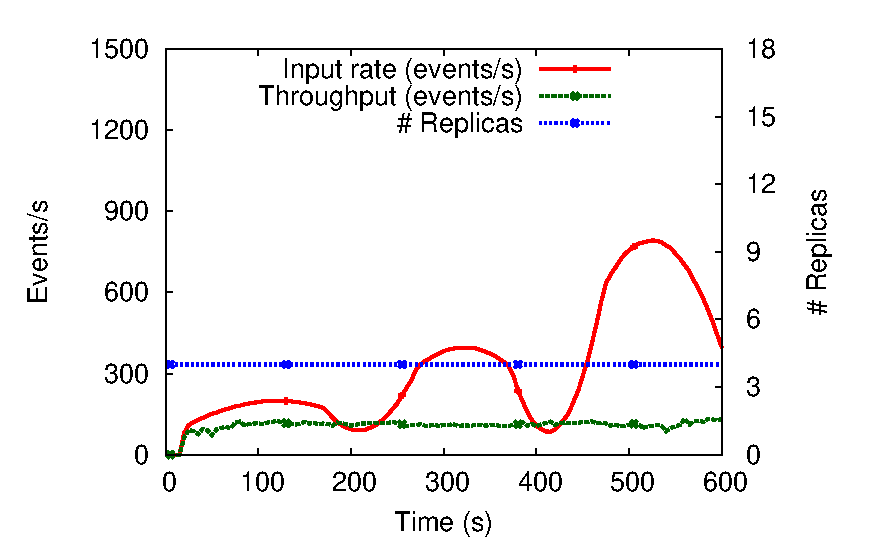
\includegraphics[scale=0.4]{images/exp/app1/dynamic/baseline/exp2-processSystem.eps}
\end{figure}
\end{multicols}
\end{frame}

\begin{frame}{Experimentos y evaluación}{Aplicación funcional - Experimento 2 - Cantidad total de eventos procesados}

\begin{itemize}
\item 201.751 eventos procesados con uso del modelo \textit{vs} 76.502 eventos procesados sin uso del modelo
\item Incremento de 2 veces la cantidad de eventos procesados
\end{itemize}

\begin{multicols}{2}
\begin{figure}[p]
	\centering
	{\scriptsize Con uso del modelo elástico\\}
	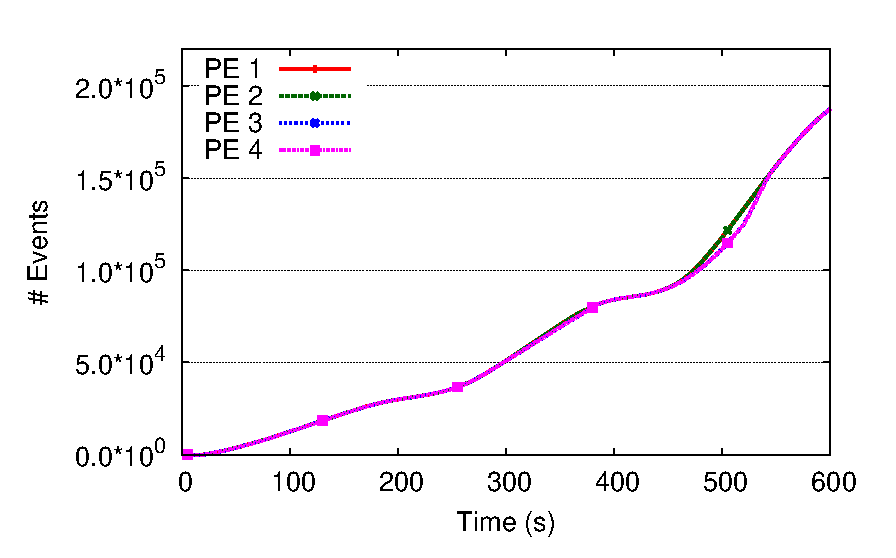
\includegraphics[scale=0.4]{images/exp/app1/dynamic/adaptative/exp2-eventCount.eps}
\end{figure}

\begin{figure}[p]
	\centering
	{\scriptsize Sin uso del modelo elástico\\}
	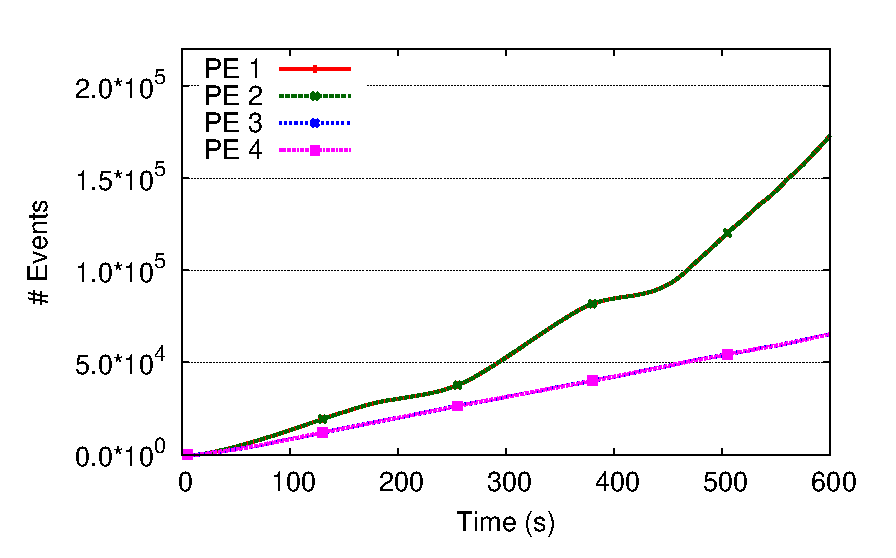
\includegraphics[scale=0.4]{images/exp/app1/dynamic/baseline/exp2-eventCount.eps}
\end{figure}
\end{multicols}
\end{frame}

%%% App 3 %%%

\begin{frame}{Experimentos y evaluación}{Aplicación sintética - Utilización promedio de CPU}

\begin{itemize}
\item $0,62\%$ promedio con uso del modelo \textit{vs} $0,61\%$ promedio sin uso del modelo
\item Aumento de un $0,01\%$ de utilización promedio de CPU
\end{itemize}

\begin{multicols}{2}
\begin{figure}[p]
	\centering
	{\scriptsize Con uso del modelo elástico\\}
	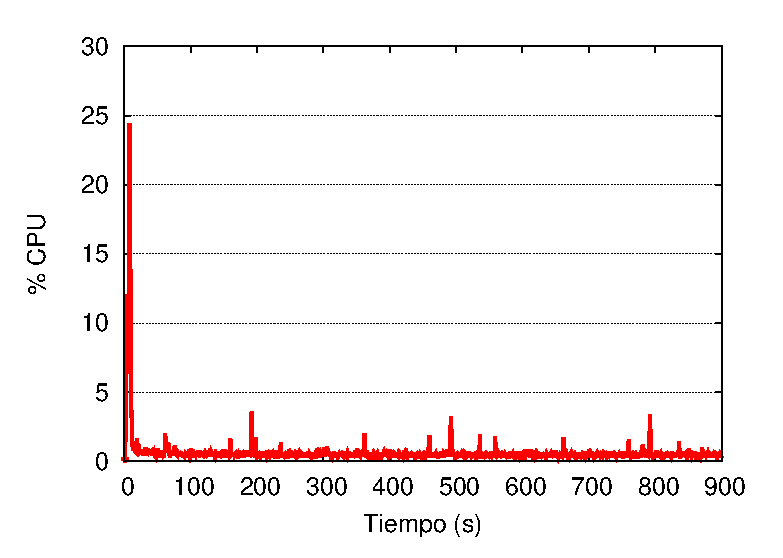
\includegraphics[scale=0.475]{images/exp/app3/cm/fisical/consumeCPU.eps}
\end{figure}

\begin{figure}[p]
	\centering
	{\scriptsize Sin uso del modelo elástico\\}
	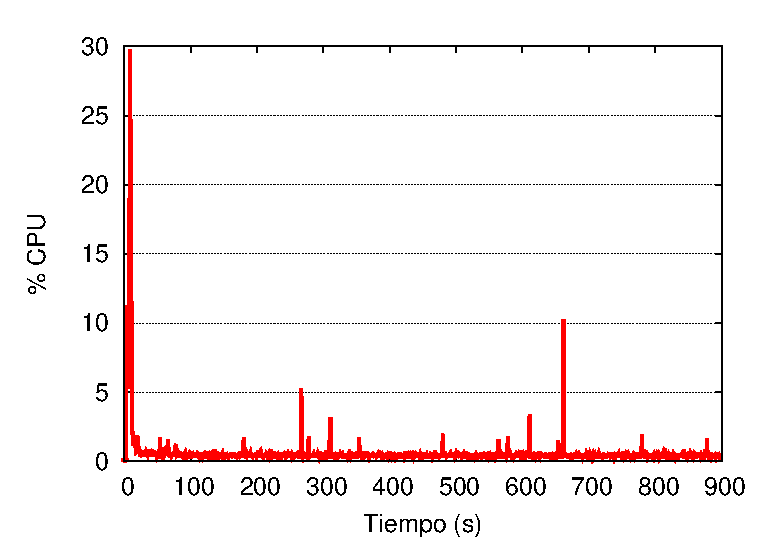
\includegraphics[scale=0.475]{images/exp/app3/sm/fisical/consumeCPU.eps}
\end{figure}
\end{multicols}
\end{frame}

\begin{frame}{Experimentos y evaluación}{Aplicación sintética - Consumo de memoria RAM}

\begin{itemize}
\item $264$MB con uso del modelo \textit{vs} $268$MB sin uso del modelo
\item Disminución de $1,5\%$ de consumo de memoria RAM
\end{itemize}

\begin{multicols}{2}
\begin{figure}[p]
	\centering
	{\scriptsize Con uso del modelo elástico\\}
	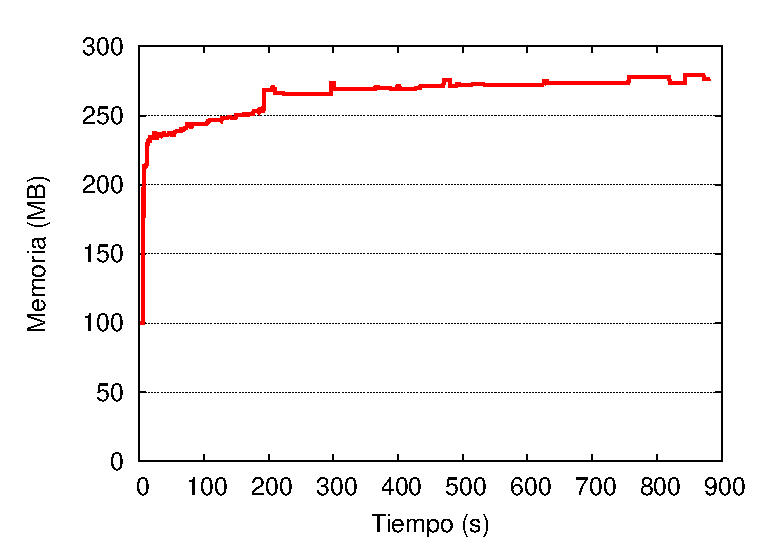
\includegraphics[scale=0.475]{images/exp/app3/cm/fisical/consumeRAM.eps}
\end{figure}

\begin{figure}[p]
	\centering
	{\scriptsize Sin uso del modelo elástico\\}
	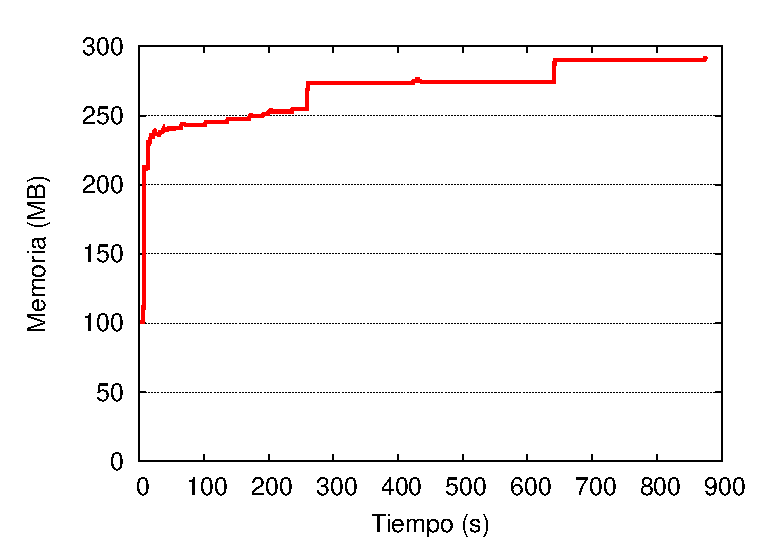
\includegraphics[scale=0.475]{images/exp/app3/sm/fisical/consumeRAM.eps}
\end{figure}
\end{multicols}
\end{frame}

\begin{frame}{Experimentos y evaluación}{Aplicación sintética - Tiempo de ejecución de cada algoritmo}
\begin{itemize}
	\item Algoritmo reactivo: 0.03 ms
	\item Algoritmo predictivo: 4.63 ms
\end{itemize}

\begin{figure}[p]
	\centering
	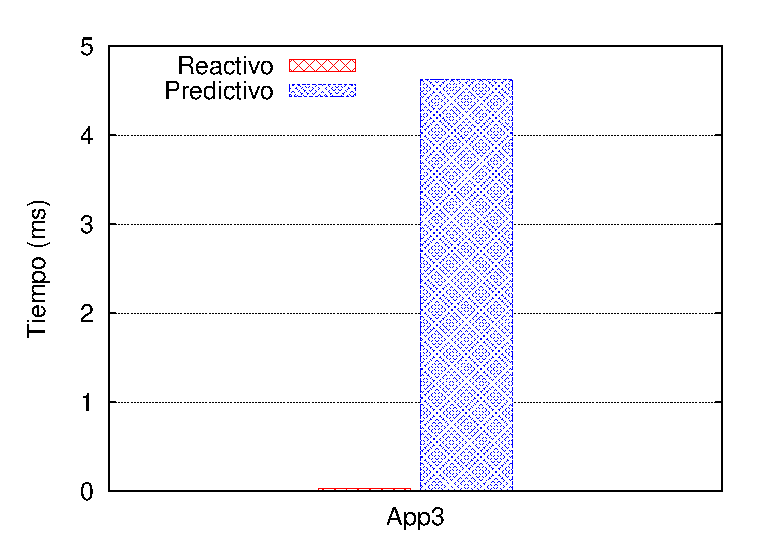
\includegraphics[scale=0.65]{images/exp/app3/cm/logical/tiempoAlgoritmos.eps}
\end{figure}

\end{frame}

\begin{frame}{Experimentos y evaluación}{Aplicación sintética - Rendimiento y cantidad de réplicas}

\begin{itemize}
\item 97 eventos/segundo con uso del modelo \textit{vs} 33 eventos/segundo sin uso del modelo
\item Incremento de 2 veces más eventos/segundo
\end{itemize}

\begin{multicols}{2}
\begin{figure}[p]
	\centering
	{\scriptsize Con uso del modelo elástico\\}
	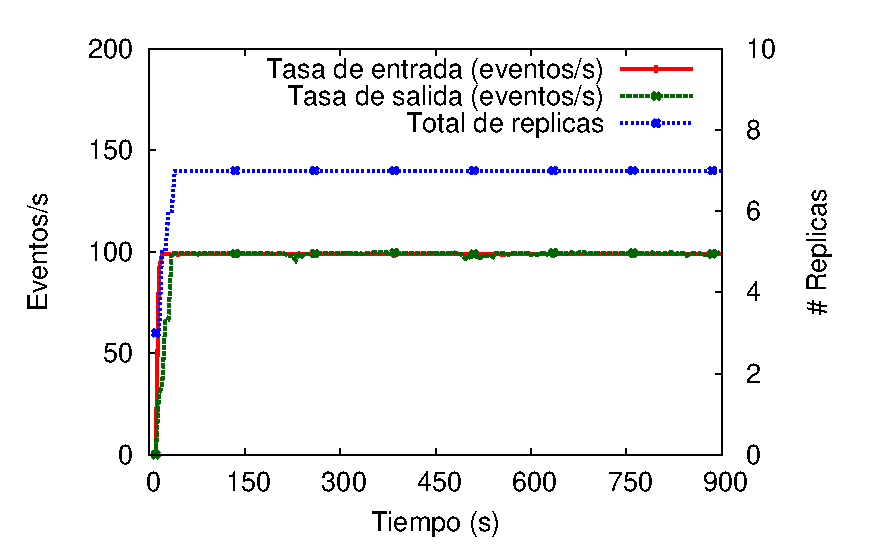
\includegraphics[scale=0.4]{images/exp/app3/cm/logical/processSystem.eps}
\end{figure}

\begin{figure}[p]
	\centering
	{\scriptsize Sin uso del modelo elástico\\}
	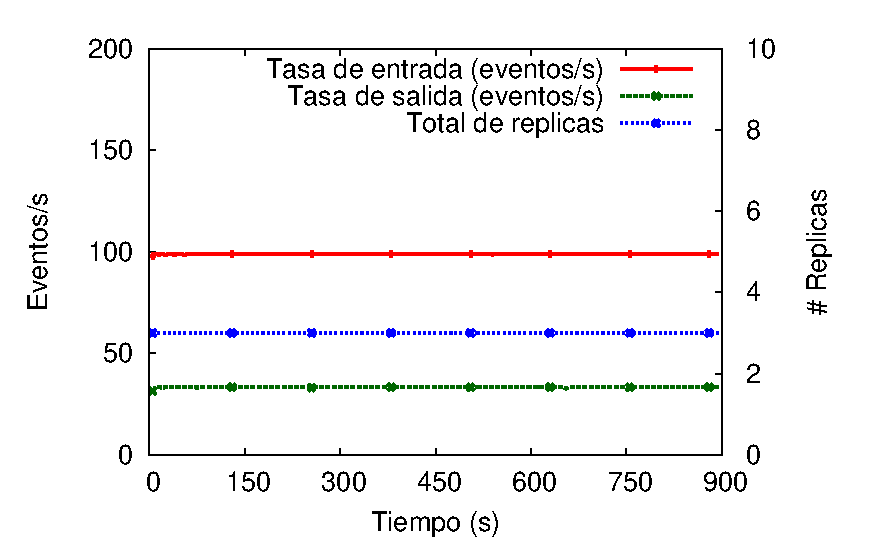
\includegraphics[scale=0.4]{images/exp/app3/sm/logical/processSystem.eps}
\end{figure}
\end{multicols}
\end{frame}

\begin{frame}{Experimentos y evaluación}{Aplicación sintética - Cantidad total de eventos procesados}

\begin{itemize}
\item 88.169 eventos procesados con uso del modelo \textit{vs} 28.714 eventos procesados sin uso del modelo
\item Incremento de 3 veces la cantidad de eventos procesados
\end{itemize}

\begin{multicols}{2}
\begin{figure}[p]
	\centering
	{\scriptsize Con uso del modelo elástico\\}
	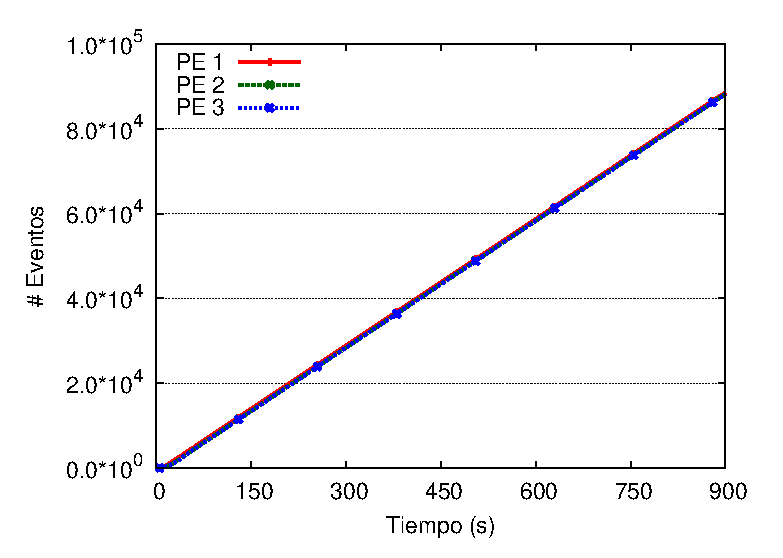
\includegraphics[scale=0.475]{images/exp/app3/cm/logical/eventCount.eps}
\end{figure}

\begin{figure}[p]
	\centering
	{\scriptsize Sin uso del modelo elástico\\}
	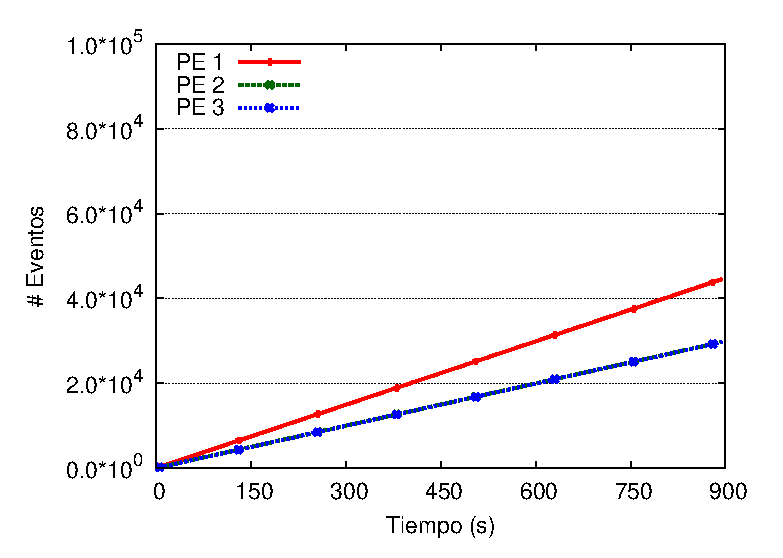
\includegraphics[scale=0.475]{images/exp/app3/sm/logical/eventCount.eps}
\end{figure}
\end{multicols}
\end{frame}
\section{Conclusiones}

\addtocounter{framenumber}{-1}
\begin{frame}[t]{Contenidos}{\textcolor{UniBlue}{.}}
	\tableofcontents[currentsection]
\end{frame}

\begin{frame}{Conclusiones}{Detalles de la contribución}

\begin{itemize}
\item Diseño e implementación de un modelo elástico
\begin{itemize}
	\item Algoritmo reactivo
	\item Algoritmo predictivo
	\item Módulo de administración de réplicas
\end{itemize}
\item Construcción de distintos escenarios $\rightarrow$ Validación del modelo diseñado
\item Evaluado y analizado el rendimiento del sistema con y sin uso del modelo elástico
\end{itemize}

\end{frame}

\begin{frame}{Conclusiones}{Discusiones}

\begin{itemize}
\item Problemas de sobrecarga en la máquina física
\begin{itemize}
	\item Procesamiento de los eventos
	\item Buffer
\end{itemize}
\item Homogeneidad de la tasa de procesamiento
\item No se realiza un análisis de los recursos físicos
\item No es capaz de detectar patrones estacionarios
\item Modelo diseñado
	\begin{itemize}
		\item Bajo cómputo
		\item Rápido análisis de los operadores
		\item Elasticidad
	\end{itemize}
\end{itemize}

\end{frame}

\begin{frame}{Conclusiones}{Trabajo a futuro}

\begin{itemize}
\item Algoritmo predictivo
\begin{itemize}
	\item Adaptabilidad del número de réplicas según el historial
	\item Machine Learning
\end{itemize}
\item Implementación en otro SPS
\end{itemize}

\end{frame}

\begin{frame}{Preguntas}{\textcolor{UniBlue}{.}}
\begin{figure}
  \center
    
\includegraphics[scale=0.25]{images/Questions.pdf}
\end{figure}
\end{frame}

\backupbegin
\begin{frame}[allowframebreaks]{Bibliografía}{\textcolor{UniBlue}{.}}
    \bibliographystyle{apalike}
    \bibliography{bibliografia.bib}
\end{frame}
\backupend

\appendix
\begin{frame}{Marco teórico}{\textcolor{UniBlue}{.}}
\begin{itemize}
	\item Ejemplo de Cadena de Markov
\end{itemize}

\begin{figure}[p]
	\centering
	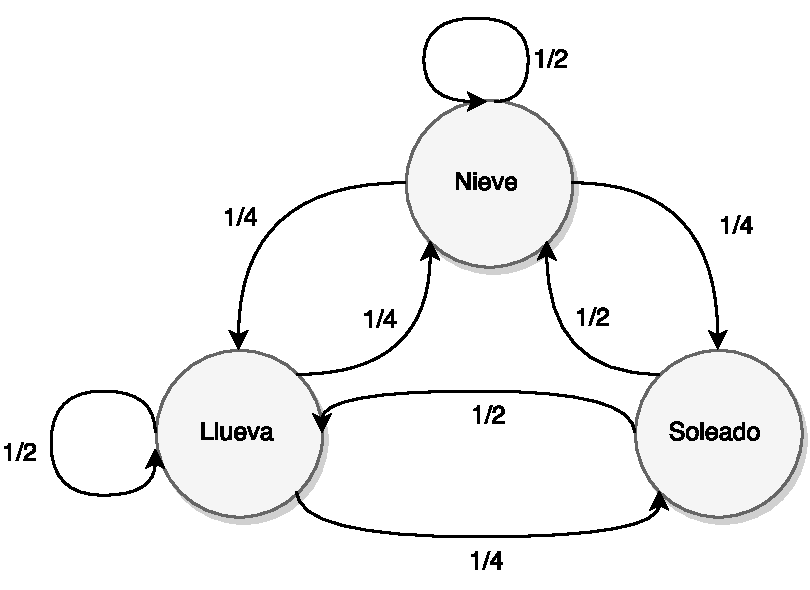
\includegraphics[scale=0.5]{images/EjCadenaMarkov.pdf}
\end{figure}

\end{frame}

\begin{frame}{Marco teórico}{\textcolor{UniBlue}{.}}
\begin{itemize}
	\item Ejemplo de Cadena de Markov reductible
\end{itemize}

\begin{figure}[p]
	\centering
	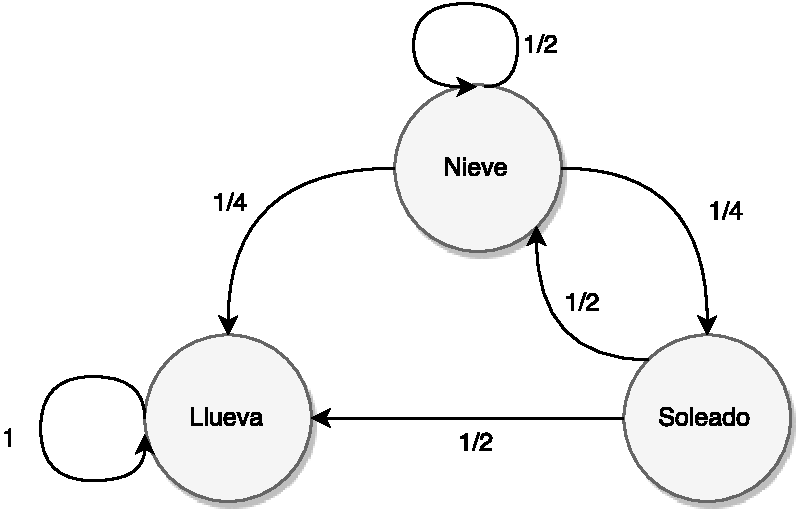
\includegraphics[scale=0.5]{images/EjCadenaMarkov-Reductible.pdf}
\end{figure}

\end{frame}

\begin{frame}{Marco teórico}{\textcolor{UniBlue}{.}}
\begin{itemize}
	\item Ejemplo de Cadena de Markov aperíodica
\end{itemize}

\begin{figure}[p]
	\centering
	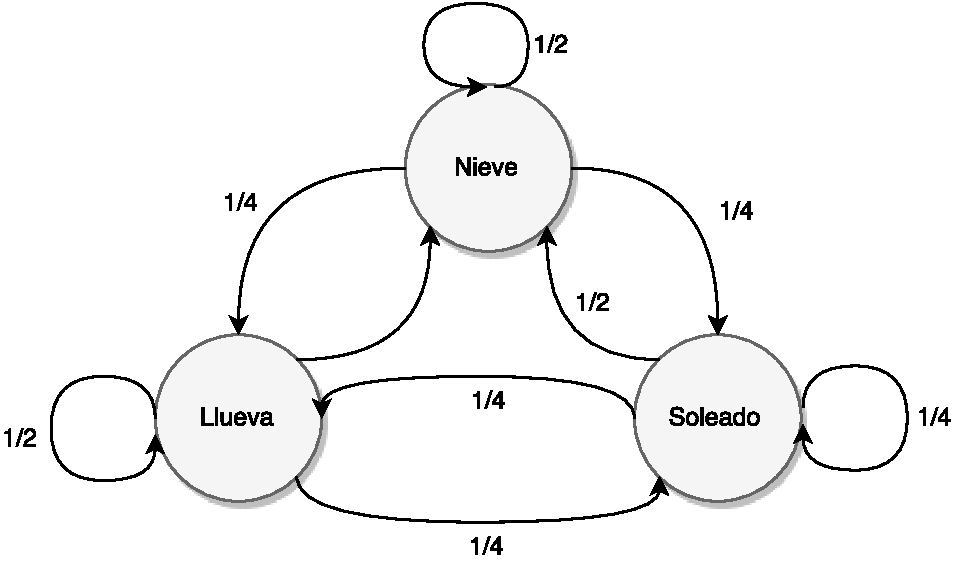
\includegraphics[scale=0.5]{images/EjCadenaMarkov-Aperiodica.pdf}
\end{figure}

\end{frame}
%%% Parámetros %%%

\begin{frame}{Experimentos y evaluación}{Parámetros}
\begin{itemize}
\item Monitor de carga
\begin{itemize}
	\item $T_m = 1seg$
\end{itemize}
\item Algoritmo reactivo
\begin{itemize}
	\item $\omega = 1$ réplica
\end{itemize} 
\item Algoritmo predictivo 
\begin{itemize}
	\item $\theta = 5$ réplicas
	\item $n = 100$ muestras
	\item $\beta = 0.25$
\end{itemize} 
\item Administrador de réplicas
\begin{itemize}
	\item Ventana de tiempo de ejecución
	\begin{itemize}
		\item $T_r = 5seg$
		\item $T_p = 100seg$
	\end{itemize}
	\item $\beta = 2$ alertas consecutivas
\end{itemize} 
\end{itemize}
\end{frame}

%%% App 1 - Constante %%%

\begin{frame}{Experimentos y evaluación}{Aplicación 1 - Constante - Rendimiento y cantidad de réplicas}

\begin{itemize}
\item 96 eventos/segundo con uso del modelo \textit{vs} 16 eventos/segundo sin uso del modelo
\item Mejora de 5 veces más eventos/segundo
\end{itemize}

\begin{multicols}{2}
\begin{figure}[p]
	\centering
	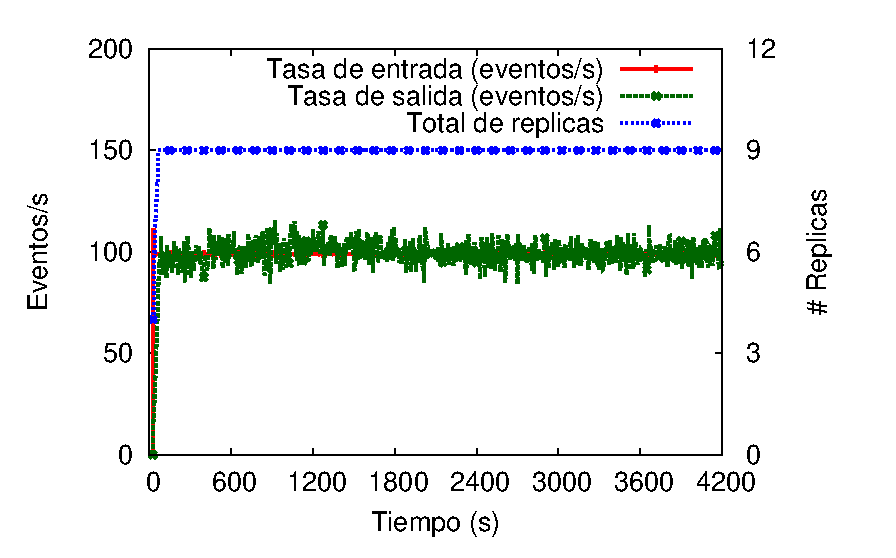
\includegraphics[scale=0.4]{images/exp/app1/uniform/cm/processSystem.eps}
\end{figure}

\begin{figure}[p]
	\centering
	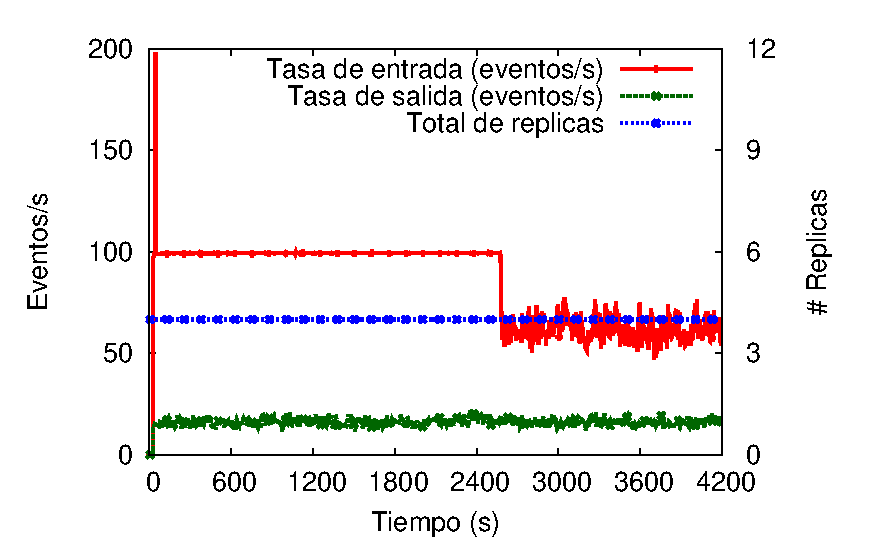
\includegraphics[scale=0.4]{images/exp/app1/uniform/sm/processSystem.eps}
\end{figure}
\end{multicols}
\end{frame}

\begin{frame}{Experimentos y evaluación}{Aplicación 1 - Constante - Cantidad total de eventos procesados}

\begin{itemize}
\item 401.618 eventos procesados con uso del modelo \textit{vs} 67.141 eventos procesados sin uso del modelo
\item Mejora de 6 veces la cantidad de eventos procesados
\end{itemize}

\begin{multicols}{2}
\begin{figure}[p]
	\centering
	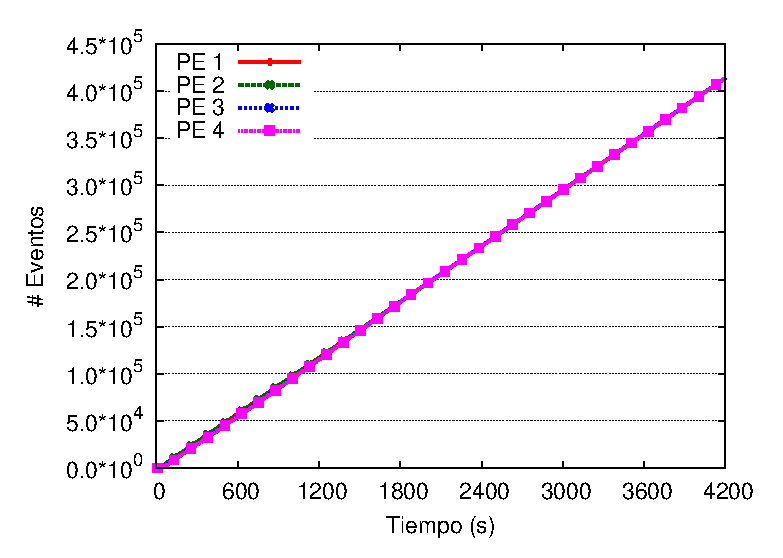
\includegraphics[scale=0.475]{images/exp/app1/uniform/cm/eventCount.eps}
\end{figure}

\begin{figure}[p]
	\centering
	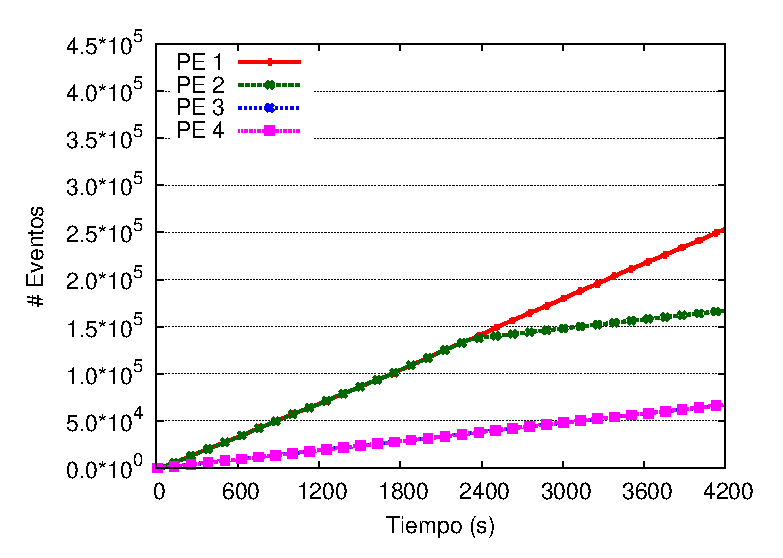
\includegraphics[scale=0.475]{images/exp/app1/uniform/sm/eventCount.eps}
\end{figure}
\end{multicols}
\end{frame}

%%% App 1 - Variable %%%

\begin{frame}{Experimentos y evaluación}{Aplicación 1 - Variable - Rendimiento y cantidad de réplicas}

\begin{itemize}
\item 72 eventos/segundo con uso del modelo \textit{vs} 19 eventos/segundo sin uso del modelo
\item Mejora de 3 veces más eventos/segundo
\end{itemize}

\begin{multicols}{2}
\begin{figure}[p]
	\centering
	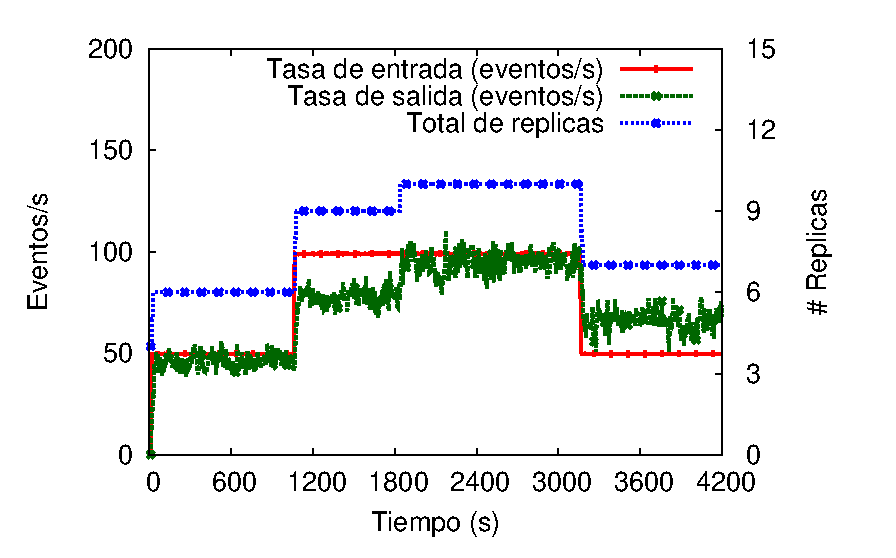
\includegraphics[scale=0.4]{images/exp/app1/normal/cm/processSystem.eps}
\end{figure}

\begin{figure}[p]
	\centering
	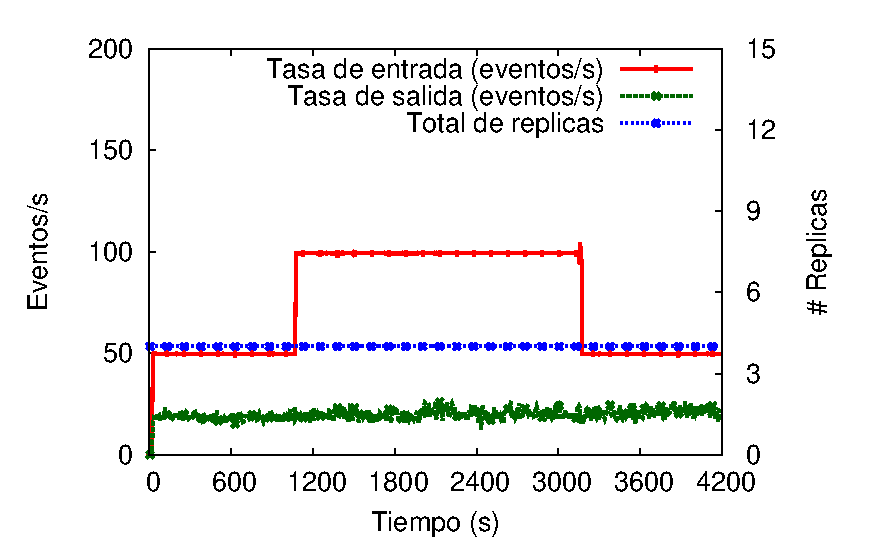
\includegraphics[scale=0.4]{images/exp/app1/normal/sm/processSystem.eps}
\end{figure}
\end{multicols}
\end{frame}

\begin{frame}{Experimentos y evaluación}{Aplicación 1 - Variable - Cantidad total de eventos procesados}

\begin{itemize}
\item 303.156 eventos procesados con uso del modelo \textit{vs} 82.770 eventos procesados sin uso del modelo
\item Mejora de 3 veces la cantidad de eventos procesados
\end{itemize}

\begin{multicols}{2}
\begin{figure}[p]
	\centering
	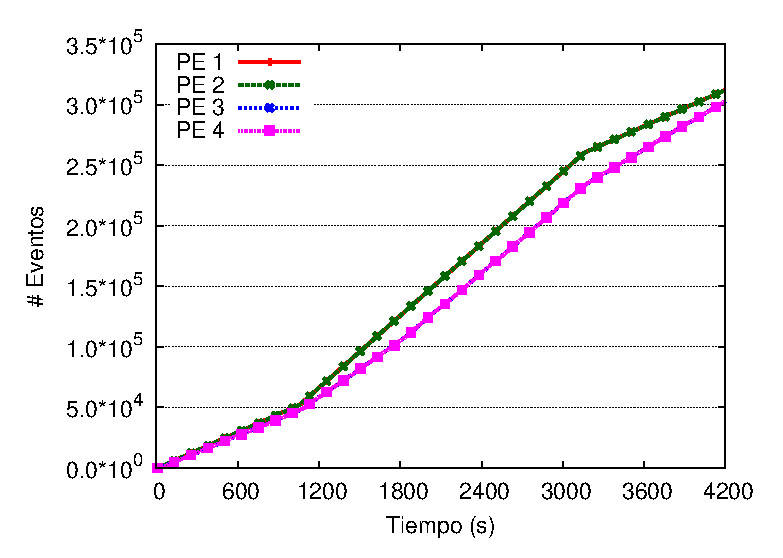
\includegraphics[scale=0.475]{images/exp/app1/normal/cm/eventCount.eps}
\end{figure}

\begin{figure}[p]
	\centering
	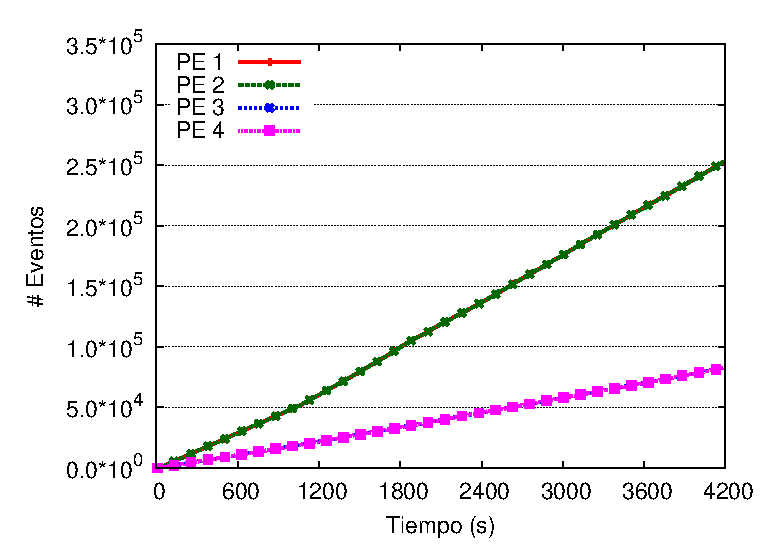
\includegraphics[scale=0.475]{images/exp/app1/normal/sm/eventCount.eps}
\end{figure}
\end{multicols}
\end{frame}

%%% App 2 - Constante %%%

\begin{frame}{Experimentos y evaluación}{Aplicación 2 - Constante - Rendimiento y cantidad de réplicas}

\begin{multicols}{2}
\begin{figure}[p]
	\centering
	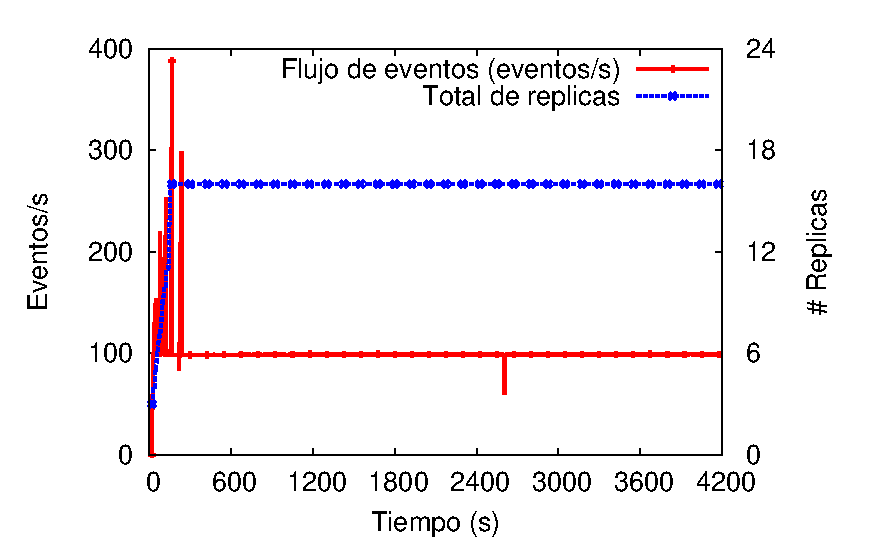
\includegraphics[scale=0.4]{images/exp/app2/uniform/cm/processSystem.eps}
\end{figure}

\begin{figure}[p]
	\centering
	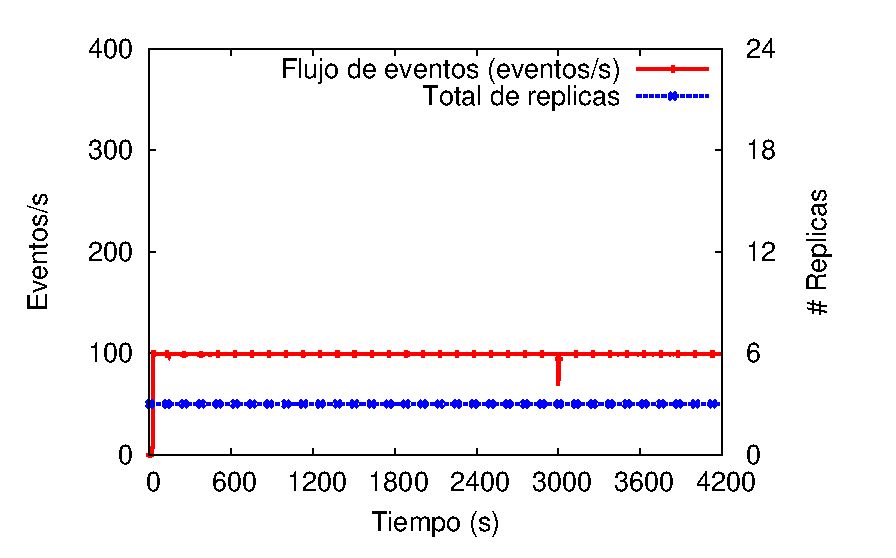
\includegraphics[scale=0.4]{images/exp/app2/uniform/sm/processSystem.eps}
\end{figure}
\end{multicols}
\end{frame}

\begin{frame}{Experimentos y evaluación}{Aplicación 2 - Constante - Cantidad total de eventos procesados}

\begin{itemize}
\item 275.290 eventos procesados con uso del modelo \textit{vs} 28.152 eventos procesados sin uso del modelo
\item Mejora de 9 veces la cantidad de eventos procesados
\end{itemize}

\begin{multicols}{2}
\begin{figure}[p]
	\centering
	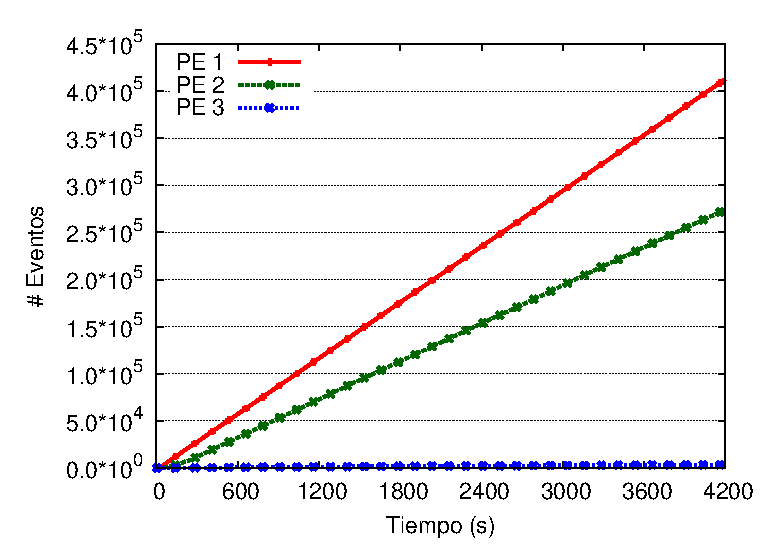
\includegraphics[scale=0.475]{images/exp/app2/uniform/cm/eventCount.eps}
\end{figure}

\begin{figure}[p]
	\centering
	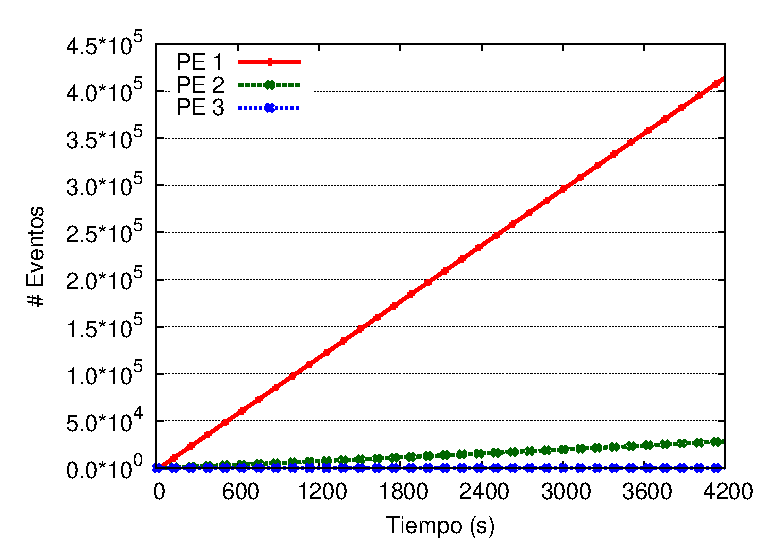
\includegraphics[scale=0.475]{images/exp/app2/uniform/sm/eventCount.eps}
\end{figure}
\end{multicols}
\end{frame}

%%% App 2 - Variable %%%

\begin{frame}{Experimentos y evaluación}{Aplicación 2 - Variable - Rendimiento y cantidad de réplicas}

\begin{multicols}{2}
\begin{figure}[p]
	\centering
	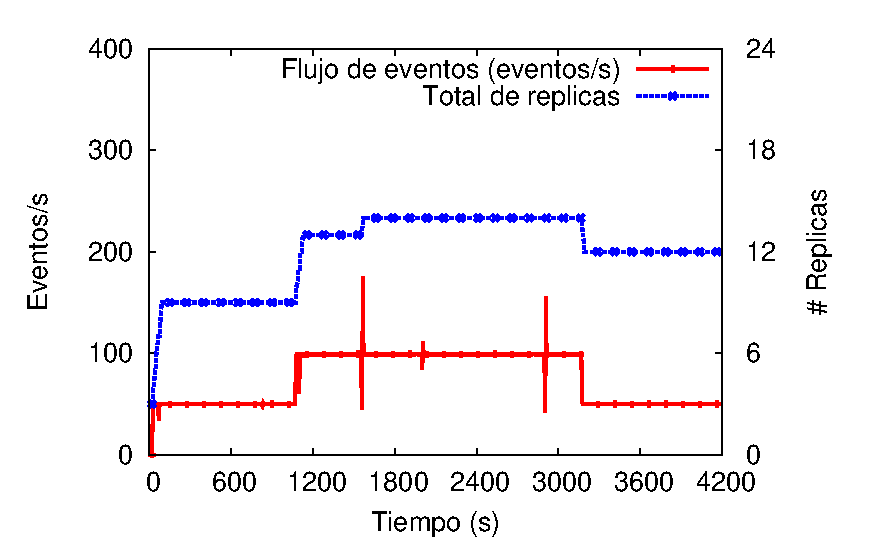
\includegraphics[scale=0.4]{images/exp/app2/normal/cm/processSystem.eps}
\end{figure}

\begin{figure}[p]
	\centering
	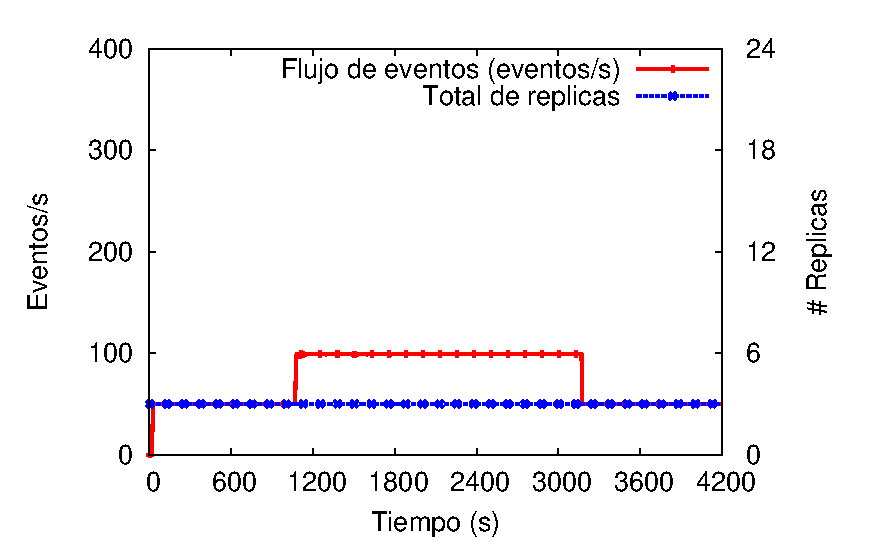
\includegraphics[scale=0.4]{images/exp/app2/normal/sm/processSystem.eps}
\end{figure}
\end{multicols}
\end{frame}

\begin{frame}{Experimentos y evaluación}{Aplicación 2 - Variable - Cantidad total de eventos procesados}

\begin{itemize}
\item 228.942 eventos procesados con uso del modelo \textit{vs} 27.751 eventos procesados sin uso del modelo
\item Mejora de 8 veces la cantidad de eventos procesados
\end{itemize}

\begin{multicols}{2}
\begin{figure}[p]
	\centering
	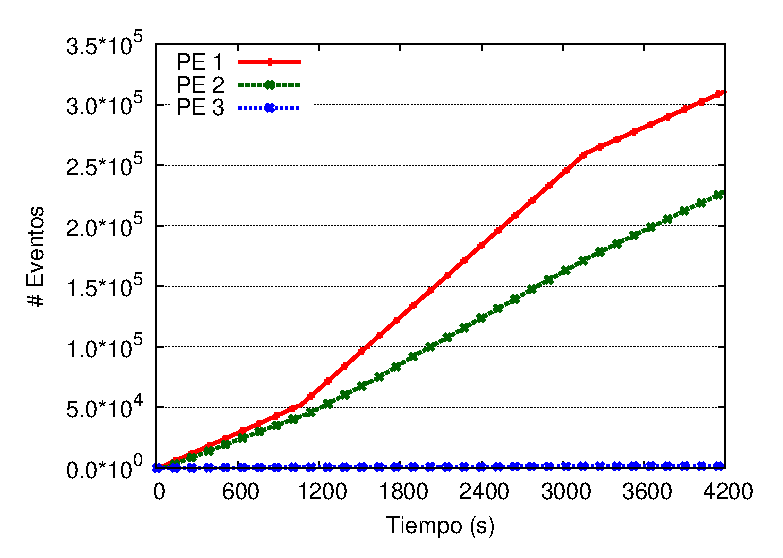
\includegraphics[scale=0.475]{images/exp/app2/normal/cm/eventCount.eps}
\end{figure}

\begin{figure}[p]
	\centering
	\includegraphics[scale=0.475]{images/exp/app2/normal/sm/eventCount.eps}
\end{figure}
\end{multicols}
\end{frame}

%%% Total de eventos procesados %%%

\begin{frame}{Experimentos y evaluación}{Cantidad de eventos procesados}

\begin{figure}[p]
	\centering
	\includegraphics[scale=0.7]{images/exp/eventTotal.eps}
\end{figure}
\end{frame}
%%% App 1 - Dynamic %%%

\begin{frame}{Experimentos y evaluación}{Aplicación funcional - Experimento 1 - Cantidad de eventos procesados}

\begin{figure}[p]
	\centering
	\includegraphics[scale=0.7]{images/exp/app1/dynamic/exp1-eventTotal.eps}
\end{figure}
\end{frame}

\begin{frame}{Experimentos y evaluación}{Aplicación funcional - Experimento 2 - Cantidad de eventos procesados}

\begin{figure}[p]
	\centering
	\includegraphics[scale=0.7]{images/exp/app1/dynamic/exp2-eventTotal.eps}
\end{figure}
\end{frame}
\begin{frame}{Twitter Stream}{\textcolor{UniBlue}{.}}
\begin{figure}
  \centering
    \includegraphics[scale=0.85]{images/appendix/streamTwitterDate.eps}
\end{figure}
\end{frame}

\end{document}